\section{Representative-consumer demand systems: linear, CES and logit}\label{sec:04-repcons}

\Cref{sec:04-spaces} showed that an unrestricted demand system in product space has far too many parameters.
One remedy imposes symmetry. A \emph{representative consumer} is a single fictitious agent whose demands equal
market demands. If she also treats all products symmetrically, a handful of parameters governs every own and
cross effect. This section develops the three systems of this kind that appear most often in applied work:
linear demand from quadratic utility, constant elasticity of substitution (CES) demand, and the logit. For each
we derive demand, elasticities, diversion and Bertrand markups. We then show that the CES and the logit are also
discrete choice models, which ties this section to the random utility models of \cref{ch:discrete}. A two-sector
version of the CES model, the model of monopolistic competition of \citet{Spence1976} and \citet{DixitStiglitz1977},
asks whether markets supply the right number of products. The section closes with the questions these systems answer
well and a table that compares them.

\subsection{Linear demand from quadratic utility}\label{sec:04-repcons-linear}

The linear demand of \cref{ex:04-linear-duopoly} has a utility foundation. A representative consumer with
income $y$ buys quantities $q_1, \dots, q_J$ of $J$ differentiated products and an amount $z$ of a numeraire good
with price one. Her utility is quasi-linear in the numeraire,
\begin{equation}\label{eq:04-quadratic-utility}
U(q, z) = z + \bar a\sum_{j=1}^J q_j - \frac{1}{2}\Big[\bar b\sum_{j=1}^J q_j^2 + 2\bar g\sum_{j<k}q_jq_k\Big],
\qquad \bar b > \bar g \ge 0
\end{equation}
\citep{SinghVives1984,Vives1999}. The parameter $\bar a$ is the marginal utility of the first unit of any
product. The parameter $\bar b$ measures how fast marginal utility falls with own consumption, and $\bar g$
measures how much consuming one product lowers the marginal utility of another. The products are substitutes
when $\bar g > 0$ and independent when $\bar g = 0$. As $\bar g$ approaches $\bar b$, utility depends only on total
consumption and the products become perfect substitutes.

\begin{proposition}[Linear demand from quadratic utility]\label{prop:04-quadratic}
Let the consumer maximize \eqref{eq:04-quadratic-utility} subject to $z + \sum_j p_jq_j = y$, and suppose the
solution has $q_j > 0$ for every $j$ and $z > 0$. Then:
\begin{enumerate}[label=(\roman*)]
\item Inverse demand is $p_j = \bar a - \bar bq_j - \bar g\sum_{k \ne j}q_k$.
\item With two products, demand is $q_j = a - bp_j + dp_k$ with
\begin{equation*}
a = \frac{\bar a}{\bar b + \bar g}, \qquad b = \frac{\bar b}{\bar b^2 - \bar g^2}, \qquad d = \frac{\bar g}{\bar b^2 - \bar g^2},
\end{equation*}
so that $b > d \ge 0$ and the diversion ratio is $D_{jk} = \frac{d}{b} = \frac{\bar g}{\bar b}$.
\item With $J$ products, for every $k \ne j$,
\begin{equation*}
\frac{\partial q_j}{\partial p_j} = -\frac{\bar b + (J-2)\bar g}{(\bar b - \bar g)[\bar b + (J-1)\bar g]},
\qquad
\frac{\partial q_k}{\partial p_j} = \frac{\bar g}{(\bar b - \bar g)[\bar b + (J-1)\bar g]},
\qquad
D_{jk} = \frac{\bar g}{\bar b + (J-2)\bar g}.
\end{equation*}
A fraction $1 - (J-1)D_{jk} = \frac{\bar b - \bar g}{\bar b + (J-2)\bar g}$ of the sales that product $j$ loses
leaves the group of products.
\end{enumerate}
\end{proposition}

\begin{proof}
For (i), substitute the budget constraint $z = y - \sum_j p_jq_j$ into utility:
\begin{equation*}
y + \sum_{j=1}^J(\bar a - p_j)q_j - \frac{1}{2}\Big[\bar b\sum_{j}q_j^2 + 2\bar g\sum_{j<k}q_jq_k\Big].
\end{equation*}
The derivative with respect to $q_j$ is $\bar a - p_j - \bar bq_j - \bar g\sum_{k\ne j}q_k$. Setting it to zero gives
(i). The Hessian of the objective is $-B$, where $B$ has $\bar b$ on the diagonal and $\bar g$ off it. In matrix form
$B = (\bar b - \bar g)I_J + \bar g\mathbf{1}\mathbf{1}^\top$. Its eigenvalues are $\bar b - \bar g > 0$ (on vectors
orthogonal to $\mathbf{1}$) and $\bar b + (J-1)\bar g > 0$ (on $\mathbf{1}$). The objective is therefore strictly
concave, and the first-order conditions characterize the maximum.

For (ii) and (iii), stack (i) as $p = \bar a\mathbf{1} - Bq$, so that $q = B^{-1}(\bar a\mathbf{1} - p)$ and
$\frac{\partial q}{\partial p^\top} = -B^{-1}$. We claim that
\begin{equation*}
B^{-1} = \frac{1}{\bar b - \bar g}\Big[I_J - \frac{\bar g}{\bar b + (J-1)\bar g}\mathbf{1}\mathbf{1}^\top\Big].
\end{equation*}
To check it, multiply by $B$ and use $\mathbf{1}\mathbf{1}^\top\mathbf{1}\mathbf{1}^\top = J\mathbf{1}\mathbf{1}^\top$:
\begin{align*}
\big[(\bar b - \bar g)I_J + \bar g\mathbf{1}\mathbf{1}^\top\big]\Big[I_J - \frac{\bar g}{\bar b + (J-1)\bar g}\mathbf{1}\mathbf{1}^\top\Big]
&= (\bar b - \bar g)I_J + \Big[\bar g - \frac{\bar g(\bar b - \bar g) + J\bar g^2}{\bar b + (J-1)\bar g}\Big]\mathbf{1}\mathbf{1}^\top \\
&= (\bar b - \bar g)I_J + \Big[\bar g - \frac{\bar g\,[\bar b + (J-1)\bar g]}{\bar b + (J-1)\bar g}\Big]\mathbf{1}\mathbf{1}^\top
= (\bar b - \bar g)I_J .
\end{align*}
The diagonal element of $-B^{-1}$ is
$-\frac{1}{\bar b - \bar g}\big[1 - \frac{\bar g}{\bar b + (J-1)\bar g}\big] = -\frac{\bar b + (J-2)\bar g}{(\bar b - \bar g)[\bar b + (J-1)\bar g]}$,
and the off-diagonal element is $\frac{\bar g}{(\bar b - \bar g)[\bar b + (J-1)\bar g]}$. This proves the derivatives in
(iii). The diversion ratio \eqref{eq:04-diversion-def} is minus their ratio. The fraction that leaves the group is
$1 - \frac{(J-1)\bar g}{\bar b + (J-2)\bar g} = \frac{\bar b - \bar g}{\bar b + (J-2)\bar g}$, which is positive
because $\bar b > \bar g$. Setting $J = 2$ gives $b = \frac{\bar b}{(\bar b - \bar g)(\bar b + \bar g)}$ and
$d = \frac{\bar g}{(\bar b - \bar g)(\bar b + \bar g)}$. The intercept is
$\frac{\bar a(\bar b - \bar g)}{\bar b^2 - \bar g^2} = \frac{\bar a}{\bar b + \bar g}$, which proves (ii).
\end{proof}

Three features of this system matter below. First, cross derivatives are symmetric,
$\frac{\partial q_k}{\partial p_j} = \frac{\partial q_j}{\partial p_k}$, because the Jacobian $-B^{-1}$ is symmetric. This
is the quasi-linear case (i) of \cref{rem:04-symmetry}. Second, the values $\bar a = 10$, $\bar b = \frac{2}{3}$ and
$\bar g = \frac{1}{3}$ give $a = 10$, $b = 2$ and $d = 1$, the numbers of \cref{ex:04-linear-duopoly}. Third, the
linear form holds only on the set of prices at which every product is bought. If $p_2$ is so high that $q_2 = 0$,
product 1 faces $q_1 = \frac{\bar a - p_1}{\bar b}$, with slope $\frac{1}{\bar b}$. This is smaller in absolute value
than $b = \frac{\bar b}{\bar b^2 - \bar g^2}$, so demand is continuous but kinked where the rival drops out.

The system has three parameters only because of symmetry. A general quadratic utility
$z + \bar a^\top q - \frac{1}{2}q^\top Bq$ with any symmetric positive definite $B$ gives the linear system
$q = B^{-1}(\bar a - p)$, with $\frac{J(J+1)}{2}$ slope parameters. That is the linear product-space system of
\cref{sec:04-spaces} with symmetry imposed. The symmetric version replaces it by $\bar b$ and $\bar g$.

\casehead{Crowded markets} The symmetric system has a strong implication for markets with many products.
Suppose $N$ single-product firms (here $N = F = J$) sell the $N$ products at a common marginal cost $c$. At
symmetric prices $p$, part (i) gives each firm the quantity $q = \frac{\bar a - p}{\bar b + (N-1)\bar g}$. By the
inverse semi-elasticity rule of \cref{sec:04-bertrand-single}, a single-product firm sets
$p - c = -q\big(\frac{\partial q_j}{\partial p_j}\big)^{-1}$. Substituting $q$ and the own slope from part (iii),
\begin{equation*}
p - c = \frac{\bar a - p}{\bar b + (N-1)\bar g}\cdot\frac{(\bar b - \bar g)[\bar b + (N-1)\bar g]}{\bar b + (N-2)\bar g}
= \frac{(\bar a - p)(\bar b - \bar g)}{\bar b + (N-2)\bar g}.
\end{equation*}
Write $\bar a - p = (\bar a - c) - (p - c)$ and collect the terms in $p - c$:
\begin{equation}\label{eq:04-linear-symmetric}
(p - c)\big[\bar b + (N-2)\bar g + \bar b - \bar g\big] = (\bar a - c)(\bar b - \bar g)
\quad\Longrightarrow\quad
p - c = \frac{(\bar a - c)(\bar b - \bar g)}{2\bar b + (N-3)\bar g}.
\end{equation}
With $N = 2$ and the numbers above, $p - c = \frac{9 \cdot \frac{1}{3}}{1} = 3$, so $p = 4$ as in
\cref{ex:04-linear-duopoly}. When $\bar g > 0$, the markup falls to zero as $N$ grows. Every new product is a
substitute for every existing one, and a crowded market approaches marginal-cost pricing. The same symmetric
products give consumers bounded gains from variety. At a common price $p$, consumer surplus is utility minus
expenditure, $Nq(\bar a - p) - \frac{1}{2}Nq^2[\bar b + (N-1)\bar g]$. Substituting $q$ gives
\begin{equation*}
CS(N) = Nq(\bar a - p) - \frac{1}{2}Nq(\bar a - p) = \frac{N(\bar a - p)^2}{2[\bar b + (N-1)\bar g]}
\;\longrightarrow\; \frac{(\bar a - p)^2}{2\bar g} \quad \text{as } N \to \infty .
\end{equation*}
The CES and logit systems behave very differently on both counts, as we show next.

\subsection{CES demand}\label{sec:04-repcons-ces}

The CES system is the workhorse of models of monopolistic competition and international trade. A representative
consumer spends income $y$ on $J$ products and has utility
\begin{equation}\label{eq:04-ces-utility}
u(q) = \Big(\sum_{j=1}^J q_j^{\frac{\sigma-1}{\sigma}}\Big)^{\frac{\sigma}{\sigma-1}}, \qquad \sigma > 1 .
\end{equation}
The parameter $\sigma$ is the \emph{elasticity of substitution}. We show below that
$\frac{q_j}{q_k} = (\frac{p_j}{p_k})^{-\sigma}$, so a one percent rise in the relative price $\frac{p_j}{p_k}$
lowers the relative quantity $\frac{q_j}{q_k}$ by $\sigma$ percent. In this section $\sigma$ always denotes the CES
elasticity, as in \cref{ch:aids}. It is a different object from the nesting parameter of the nested logit, which
other chapters also write as $\sigma$. Two other conventions appear in the literature. Some authors write the
inner exponent as $\varsigma = \frac{\sigma - 1}{\sigma} \in (0,1)$, so that $\sigma = \frac{1}{1-\varsigma}$. Others use a different
outer exponent, such as $(\sum_j q_j^\varsigma)^{1-\varsigma}$. Any strictly increasing transformation of $u$ represents the same
preferences, so all of these forms give the same demand.

\begin{proposition}[CES demand and Bertrand pricing]\label{prop:04-ces}
Let the consumer maximize \eqref{eq:04-ces-utility} subject to $\sum_j p_jq_j = y$. Define the \emph{CES price index}
$P^{CES} = \big(\sum_{k=1}^J p_k^{1-\sigma}\big)^{\frac{1}{1-\sigma}}$ and the expenditure shares
$s_j = \frac{p_jq_j}{y}$. Then:
\begin{enumerate}[label=(\roman*)]
\item Demand is
\begin{equation}\label{eq:04-ces-demand}
q_j = \frac{p_j^{-\sigma}}{\sum_{k}p_k^{1-\sigma}}\,y = \Big(\frac{p_j}{P^{CES}}\Big)^{-\sigma}\frac{y}{P^{CES}},
\qquad
s_j = \Big(\frac{p_j}{P^{CES}}\Big)^{1-\sigma},
\end{equation}
and indirect utility is $\frac{y}{P^{CES}}$.
\item The own elasticity is $\varepsilon_j = \sigma - (\sigma - 1)s_j = \sigma(1 - s_j) + s_j$, the cross elasticity
is $\varepsilon_{jk} = (\sigma - 1)s_k$ for $k \ne j$, and the income elasticity is one.
\item The diversion ratio is $D_{jk} = \frac{(\sigma - 1)p_jq_k}{y[\sigma - (\sigma - 1)s_j]}$. Measured in
expenditure, the fraction of the revenue lost by $j$ that goes to $k$ is
$-\frac{\partial(p_kq_k)}{\partial p_j}\big(\frac{\partial(p_jq_j)}{\partial p_j}\big)^{-1} = \frac{s_k}{1 - s_j}$.
\item Suppose each product has constant marginal cost $mc_j$ and firms set prices as in \cref{sec:04-bertrand}. A
single-product firm sets
\begin{equation}\label{eq:04-ces-lerner}
\frac{p_j - mc_j}{p_j} = \frac{1}{\sigma - (\sigma - 1)s_j}.
\end{equation}
A firm that sells the products $\mathcal{J}_f$ gives all of them the same Lerner index,
$\frac{p_j - mc_j}{p_j} = \frac{1}{\sigma - (\sigma - 1)S_f}$, where $S_f = \sum_{k\in\mathcal{J}_f}s_k$.
\end{enumerate}
\end{proposition}

\begin{proof}
(i) Let $\varsigma = \frac{\sigma - 1}{\sigma} \in (0,1)$ and $V(q) = \sum_j q_j^\varsigma$. Since $u = V^{\frac{1}{\varsigma}}$ is a strictly
increasing function of $V$, we may maximize $V$. It is strictly concave, and its marginal utilities are infinite at
zero, so the solution is interior and unique. The first-order condition of the Lagrangian is
$\varsigma q_j^{\varsigma-1} = \lambda p_j$. Since $\varsigma - 1 = -\frac{1}{\sigma}$, it gives
\begin{equation*}
q_j = \Big(\frac{\lambda}{\varsigma}\Big)^{-\sigma}p_j^{-\sigma} \equiv Cp_j^{-\sigma},
\end{equation*}
with $C$ the same for all products. The budget constraint gives $\sum_j p_j\,Cp_j^{-\sigma} = C\sum_j p_j^{1-\sigma} = y$,
so $C = \frac{y}{\sum_k p_k^{1-\sigma}}$. By definition $\sum_k p_k^{1-\sigma} = (P^{CES})^{1-\sigma}$, hence
$q_j = p_j^{-\sigma}(P^{CES})^{\sigma-1}y$, which is \eqref{eq:04-ces-demand}. Multiplying by $\frac{p_j}{y}$ gives
the share. For indirect utility, note that $\sigma\varsigma = \sigma - 1$, so
\begin{equation*}
q_j^\varsigma = \Big(\frac{p_j}{P^{CES}}\Big)^{-\sigma\varsigma}\Big(\frac{y}{P^{CES}}\Big)^\varsigma
= \Big(\frac{p_j}{P^{CES}}\Big)^{1-\sigma}\Big(\frac{y}{P^{CES}}\Big)^\varsigma = s_j\Big(\frac{y}{P^{CES}}\Big)^\varsigma .
\end{equation*}
Summing over $j$ gives $V = (\frac{y}{P^{CES}})^\varsigma$, so $u = \frac{y}{P^{CES}}$. \Cref{prop:05-ces} derives the
expenditure function and the other duality relations.

(ii) Take logs of \eqref{eq:04-ces-demand}: $\ln q_j = -\sigma\ln p_j + (\sigma - 1)\ln P^{CES} + \ln y$. From
$\ln P^{CES} = \frac{1}{1-\sigma}\ln\sum_k p_k^{1-\sigma}$,
\begin{equation*}
\frac{\partial\ln P^{CES}}{\partial\ln p_k} = \frac{1}{1-\sigma}\cdot\frac{(1-\sigma)p_k^{1-\sigma}}{\sum_l p_l^{1-\sigma}} = s_k .
\end{equation*}
Hence $\frac{\partial\ln q_j}{\partial\ln p_j} = -\sigma + (\sigma - 1)s_j$, $\frac{\partial\ln q_j}{\partial\ln p_k} = (\sigma - 1)s_k$
and $\frac{\partial\ln q_j}{\partial\ln y} = 1$. The own elasticity, written as a positive number, is
$\varepsilon_j = \sigma - (\sigma - 1)s_j$.

(iii) By (ii), $\frac{\partial q_k}{\partial p_j} = (\sigma - 1)s_j\frac{q_k}{p_j}$ and
$\frac{\partial q_j}{\partial p_j} = -\varepsilon_j\frac{q_j}{p_j}$. Their ratio is
\begin{equation*}
D_{jk} = \frac{(\sigma - 1)s_jq_k}{\varepsilon_jq_j} = \frac{(\sigma - 1)p_jq_k}{y[\sigma - (\sigma - 1)s_j]},
\end{equation*}
because $\frac{s_j}{q_j} = \frac{p_j}{y}$. For revenues, $\frac{\partial(p_jq_j)}{\partial p_j} = q_j(1 - \varepsilon_j) = -(\sigma - 1)(1 - s_j)q_j$
and $\frac{\partial(p_kq_k)}{\partial p_j} = p_k\frac{\partial q_k}{\partial p_j} = (\sigma - 1)\frac{s_js_ky}{p_j}$. Their ratio, with a minus
sign, is $\frac{s_js_ky}{p_jq_j(1 - s_j)} = \frac{s_k}{1 - s_j}$, since $p_jq_j = s_jy$.

(iv) For a single-product firm, the inverse elasticity rule of \cref{sec:04-bertrand-single} gives
$\frac{p_j - mc_j}{p_j} = \frac{1}{\varepsilon_j}$, and $\varepsilon_j - 1 = (\sigma - 1)(1 - s_j) > 0$. For a
multi-product firm, write the first-order condition \eqref{eq:04-foc-scalar} for $j \in \mathcal{J}_f$ and substitute
the derivatives from (iii):
\begin{equation*}
q_j - (p_j - mc_j)\varepsilon_j\frac{q_j}{p_j} + \sum_{k\in\mathcal{J}_f\setminus\{j\}}(p_k - mc_k)(\sigma - 1)s_j\frac{q_k}{p_j} = 0 .
\end{equation*}
Let $L_k = \frac{p_k - mc_k}{p_k}$, so that $(p_k - mc_k)q_k = L_ks_ky$. Divide by $q_j$ and use $\frac{s_jy}{p_jq_j} = 1$:
\begin{equation*}
1 - L_j\varepsilon_j + (\sigma - 1)\sum_{k\in\mathcal{J}_f\setminus\{j\}}L_ks_k = 0 .
\end{equation*}
Substitute $\varepsilon_j = \sigma - (\sigma - 1)s_j$ and move the term $(\sigma - 1)L_js_j$ into the sum:
\begin{equation*}
\sigma L_j = 1 + (\sigma - 1)\sum_{k\in\mathcal{J}_f}L_ks_k .
\end{equation*}
The right side is the same for every $j \in \mathcal{J}_f$, so the firm's products share one Lerner index $L_f$.
Then $\sigma L_f = 1 + (\sigma - 1)S_fL_f$, and solving gives $L_f = \frac{1}{\sigma - (\sigma - 1)S_f}$.
\end{proof}

Part (ii) shows how little freedom the system has. One parameter governs all substitution. The own elasticity is
a weighted average of $\sigma$ and one, with weight $s_j$ on the unit elasticity of total spending. When $p_k$ rises,
every other product gains demand in the same proportion, $(\sigma - 1)s_k$, however close it is to $k$. With many
small products every own elasticity is close to $\sigma$. Part (iii) restates this in the language of
\cref{sec:04-diversion}. Quantity diversion is proportional to $q_k$, and expenditure diversion is exactly the logit
formula $\frac{s_k}{1 - s_j}$. The quantity ratios do not sum to one, because total spending is fixed while total
units are not.

\casehead{Symmetric firms and the large-group limit} Let $N$ single-product firms ($N = F = J$) share a common
marginal cost. In the symmetric equilibrium $s_j = \frac{1}{N}$, and \eqref{eq:04-ces-lerner} becomes
\begin{equation}\label{eq:04-ces-symmetric}
\frac{p - mc}{p} = \frac{1}{\sigma - \frac{\sigma - 1}{N}} = \frac{N}{\sigma N - \sigma + 1}.
\end{equation}
The Lerner index equals $\frac{2}{\sigma + 1}$ with two firms and falls toward $\frac{1}{\sigma}$ as $N$ grows. In the
limit $p = \frac{\sigma}{\sigma - 1}mc$, the constant markup of monopolistic competition in the model of
\citet{DixitStiglitz1977}. There each firm is too small to affect $P^{CES}$, so it perceives the elasticity $\sigma$.
\Citet{CaplinNalebuff1991} note (footnote 19) that an early version of the Dixit-Stiglitz paper worked with a
continuum of firms, for which this own effect is exactly zero. With finitely many firms it is positive, and
with few firms ignoring it is inappropriate. The exact formula measures the error. With $\sigma = 3$ and $N = 10$
the Lerner index is $\frac{1}{2.8} = 0.357$, against $\frac{1}{3} = 0.333$ in the large-group approximation.

The case $N = 1$ shows why at least two firms are needed. A single seller has $s = 1$ and faces unit-elastic demand
$q = \frac{y}{p}$. Its revenue is fixed at $y$. With $mc > 0$, its profit $y - mc\,\frac{y}{p}$ rises with $p$ toward
the supremum $y$, which no finite price attains, so no finite price is optimal. With $mc = 0$ every price earns $y$,
so the price is indeterminate. With $N \ge 2$ each firm's demand is log-concave in the logarithm of its own price.
By part (ii), the elasticity $\sigma - (\sigma - 1)s_j$ rises with $p_j$ because $s_j$ falls. The log-log
condition of \cref{sec:04-existence-demand} then makes profit quasi-concave in own price. \Citet{CaplinNalebuff1991}
prove that a pure-strategy equilibrium exists with at least two firms and positive costs, and that it is unique in
the duopoly (\cref{sec:04-repcons-cesdc}).

\casehead{Why CES misleads for mergers} Part (iv) says that a CES firm's markup depends only on its combined
expenditure share. A merger of products $j$ and $k$ raises both Lerner indices to
$\frac{1}{\sigma - (\sigma - 1)(s_j + s_k)}$ at given shares. Nothing in this formula refers to how close $j$ and $k$
are. Two near-identical brands and two unrelated products with the same shares produce the same predicted price
increase. A numerical illustration makes the point. Take ten single-product firms with $mc = 1$ and $\sigma = 3$.
In the symmetric equilibrium each has share 0.1, Lerner index 0.357 and price 1.556. Now let firms 1 and 2 merge.
We solve the post-merger first-order conditions of part (iv) by iterating on the Lerner formulas. The merged
firm raises both prices by 3.9 percent, to 1.616, and each of its products' shares falls to 0.094. Each rival raises
its price by 0.06 percent. These predictions hold for every pair of firms, whether the merging products are close or
distant substitutes. The model has no parameter that could tell the two cases apart. For the same reason CES
markups are nearly equal across products whenever shares are small, whatever the pattern of competition.

\begin{remark}[Taste weights and an outside good]\label{rem:04-ces-weights}
\Cref{ch:aids} writes CES utility with weights,
$u(q) = \big(\sum_j a_j^{\frac{1}{\sigma}}q_j^{\frac{\sigma-1}{\sigma}}\big)^{\frac{\sigma}{\sigma-1}}$ with $a_j > 0$
(\cref{prop:05-ces}). The weights act as quality shifters. They change the price index to
$P^{CES} = \big(\sum_k a_kp_k^{1-\sigma}\big)^{\frac{1}{1-\sigma}}$ and the shares to
$s_j = a_j\big(\frac{p_j}{P^{CES}}\big)^{1-\sigma}$. Parts (ii) to (iv) of \cref{prop:04-ces} hold unchanged when
written in terms of these shares. An outside good can be added through a Cobb-Douglas upper tier in $u(q)$ and a
numeraire. The consumer then spends a fixed fraction of income on the differentiated products, and every result
holds with $y$ replaced by that expenditure \citep[Section 8]{CaplinNalebuff1991}.
\end{remark}

\subsection{The logit as the demand of a representative consumer}\label{sec:04-repcons-logit}

The logit is usually derived from a population of consumers with random utility (\cref{ch:discrete}).
\citet{AndersonDePalmaThisse1988} show that the same shares solve the problem of a single consumer with a taste for
variety. Write mean utility as $\delta_j = \tilde\delta_j - \alpha p_j$, where $\tilde\delta_j = x_j\beta + \xi_j$ is
the quality of product $j$ before price is taken into account. The outside good has $\tilde\delta_0 = p_0 = 0$. The
consumer allocates one unit of consumption across the $J + 1$ alternatives, so $q_j$ is the fraction of the unit
that goes to alternative $j$. With a market of size one, $q_j$ is also the market share.

\begin{proposition}[Logit demand from an entropy representative consumer]\label{prop:04-logit-entropy}
Consider the program, with the convention $0\ln 0 = 0$,
\begin{equation}\label{eq:04-entropy}
\max_{q_0, \dots, q_J \ge 0}\; \sum_{j=0}^J(\tilde\delta_j - \alpha p_j)q_j - \sum_{j=0}^J q_j\ln q_j
\qquad\text{subject to}\qquad \sum_{j=0}^J q_j = 1 .
\end{equation}
\begin{enumerate}[label=(\roman*)]
\item The program has a unique solution. It is interior and equals the logit shares
$q_j = \frac{e^{\delta_j}}{\Phi}$, with $\Phi = 1 + \sum_{k=1}^J e^{\delta_k}$.
\item The maximized value is $\ln\Phi$.
\item The same demands solve the quasi-linear program
$\max\; y - \sum_j p_jq_j + \frac{1}{\alpha}\big[\sum_j\tilde\delta_jq_j - \sum_j q_j\ln q_j\big]$ subject to
$\sum_j q_j = 1$. Its maximized value is $y + \frac{1}{\alpha}\ln\Phi$, and the derivative of this value with respect
to $p_j$ equals $-q_j$.
\end{enumerate}
\end{proposition}

\begin{proof}
(i) The objective is continuous on the simplex, which is compact, so a maximum exists. The function
$-q\ln q$ is strictly concave and the other terms are linear, so the objective is strictly concave and the maximum
is unique. The derivative of $-q\ln q$ is $-\ln q - 1$, which tends to $+\infty$ as $q \to 0$. Moving a little
mass from any alternative with positive consumption to one with zero consumption therefore raises the objective.
The maximum is interior, and it solves the first-order conditions of the Lagrangian
$\sum_j\delta_jq_j - \sum_jq_j\ln q_j - \lambda(\sum_j q_j - 1)$:
\begin{equation*}
\delta_j - \ln q_j - 1 - \lambda = 0
\quad\Longrightarrow\quad
q_j = e^{\delta_j}e^{-(1+\lambda)} .
\end{equation*}
The constraint gives $e^{-(1+\lambda)}\sum_{k=0}^J e^{\delta_k} = 1$. Since $\delta_0 = 0$, the sum equals $\Phi$, and
$q_j = \frac{e^{\delta_j}}{\Phi}$.

(ii) At the solution $\ln q_j = \delta_j - \ln\Phi$. The value is
$\sum_j\delta_jq_j - \sum_jq_j(\delta_j - \ln\Phi) = \ln\Phi\sum_jq_j = \ln\Phi$.

(iii) Since $-\sum_j p_jq_j = \frac{1}{\alpha}\sum_j(-\alpha p_j)q_j$, the quasi-linear objective equals $y$ plus
$\frac{1}{\alpha}$ times the objective in \eqref{eq:04-entropy}. It has the same maximizer and the value
$y + \frac{1}{\alpha}\ln\Phi$. Finally, $\frac{\partial}{\partial p_j}\frac{1}{\alpha}\ln\Phi = \frac{1}{\alpha}\cdot\frac{-\alpha e^{\delta_j}}{\Phi} = -q_j$.
\end{proof}

The adding-up constraint does the work of substitution. Without it, the first-order conditions read
$\delta_j - \ln q_j - 1 = 0$ and give $q_j = e^{\delta_j - 1}$. Each demand would then depend only on its own
price, and no product would gain when a rival raised its price. The constraint ties the demands together through
the multiplier $\lambda$, which equals the inclusive value $\ln\Phi$ minus one.

The term $-\sum_jq_j\ln q_j$ is the \emph{entropy} of the consumption profile. It is largest when consumption is
spread evenly, so it represents a taste for variety. In the quasi-linear form of part (iii) the entropy carries
the weight $\frac{1}{\alpha}$, and $\frac{\tilde\delta_j}{\alpha}$ is the dollar value of product $j$'s quality. As
$\alpha$ grows, the taste for variety vanishes relative to money. The consumer then concentrates on the alternative
with the largest net value $\frac{\tilde\delta_j}{\alpha} - p_j$, as buyers of a homogeneous good would. As $\alpha$
falls, variety dominates and consumption spreads out.

The proposition gives the logit two foundations with the same aggregate demand. In the population view, consumer
$i$ has utility $u_{ij} = \delta_j + \epsilon_{ij}$ with i.i.d.\ type-I extreme value shocks and buys one unit of her
best alternative \citep{McFadden1974}. Her expected maximum utility is $\ln\Phi$ plus Euler's constant
(\cref{ch:discrete}). Part (ii) shows that the representative consumer's value has the same form. The log-sum
measure of consumer surplus used in \cref{ch:logit} therefore has a representative-consumer reading as well. Part
(iii) is a version of Roy's identity: the derivative of the value with respect to a price is minus the demand.

\begin{remark}[Perturbed utility and random utility]\label{rem:04-perturbed}
The equivalence extends beyond the logit. Take any additive random utility model with a strictly positive joint
density of shocks and continuously differentiable choice probabilities. Its choice probabilities maximize
$\sum_j\delta_jq_j - \mathcal{C}(q)$ over the interior of the simplex for some function $\mathcal{C}(q)$
\citep[Theorem~2.1, p.~2269]{HofbauerSandholm2002}. This $\mathcal{C}$ is strictly convex on the interior of the simplex, and its gradient grows without
bound near the boundary. For the logit, $\mathcal{C}$ is the negative entropy $\sum_jq_j\ln q_j$. The converse fails. With four
or more alternatives, no additive random utility model generates the demands that maximize
$\sum_j\delta_jq_j + \sum_j\ln q_j$ \citep[Proposition~2.2, p.~2271]{HofbauerSandholm2002}.
\end{remark}

\casehead{IIA, elasticities and diversion} At the solution, $\frac{q_j}{q_k} = e^{\delta_j - \delta_k}$ depends only on
products $j$ and $k$. This is the independence of irrelevant alternatives (IIA). The derivatives
\eqref{eq:04-logit-derivs} give $\varepsilon_j = \alpha p_j(1 - s_j)$, $\varepsilon_{kj} = \alpha p_js_j$ for every $k \ne j$,
and $D_{jk} = \frac{s_k}{1 - s_j}$ (\cref{sec:04-diversion-systems}). The classic illustration is the red bus and the
blue bus. A commuter chooses between a car and a red bus, each with share $\frac{1}{2}$. Now add a blue bus that
is identical to the red one. Intuition says the car keeps $\frac{1}{2}$ and the buses split the other half. The
logit gives each option $\frac{1}{3}$, because it treats the blue bus as a new product with its own taste shock
(\cref{ch:logit}). The entropy view tells the same story. The representative consumer gains $\ln 3 - \ln 2$ utils
from the duplicate, because the entropy term rewards variety itself. This is the ``too many characteristics''
problem of \cref{sec:04-spaces-drawbacks}.

Logit and CES share the same proportional substitution, and both allow quality differences ($\tilde\delta_j$ in
the logit, the weights $a_j$ of \cref{rem:04-ces-weights} in the CES). They differ in what is held fixed and in how
price enters. In the logit, total quantity is fixed and price enters utility in levels. In the CES, total spending
is fixed and price enters through its logarithm, as the next subsection shows. As a result, logit markups are
constant in dollars for a given share, $\frac{1}{\alpha(1 - s_j)}$. CES markups are constant as a fraction of price,
$\frac{1}{\sigma - (\sigma - 1)s_j}$.

\subsection{CES as a discrete choice model*}\label{sec:04-repcons-cesdc}

The CES demand of a representative consumer can also be generated by a population in which each consumer buys only
one product \citep{AndersonDePalmaThisse1987}. Let a mass $M$ of consumers each have income $y$. Consumer $i$ picks
one product and spends all of her income on it, so she buys $\frac{y}{p_j}$ units if she picks $j$. Her utility from
$q$ units of product $j$ is $\ln q + \frac{1}{\sigma - 1}\epsilon_{ij}$, so her indirect utility from choosing $j$ is
\begin{equation}\label{eq:04-ces-rum}
u_{ij} = \ln y - \ln p_j + \frac{1}{\sigma - 1}\epsilon_{ij},
\end{equation}
with $\epsilon_{ij}$ i.i.d.\ type-I extreme value across consumers and products.

\begin{proposition}[CES as a discrete choice model]\label{prop:04-ces-discrete}
Under \eqref{eq:04-ces-rum}, with $\sigma > 1$:
\begin{enumerate}[label=(\roman*)]
\item The probability that a consumer chooses $j$ is $\frac{p_j^{1-\sigma}}{\sum_k p_k^{1-\sigma}}$. This is a logit
in $-\ln p_j$ with coefficient $\sigma - 1$, and it equals the CES expenditure share of \eqref{eq:04-ces-demand}.
\item Expected demand for product $j$ is $\frac{My\,p_j^{-\sigma}}{\sum_k p_k^{1-\sigma}}$, the CES demand of a
representative consumer with income $My$ and elasticity of substitution $\sigma$.
\item Expected maximum utility is $\E[\max_j u_{ij}] = \ln\frac{y}{P^{CES}} + \frac{\gamma_E}{\sigma - 1}$, where
$\gamma_E \approx 0.5772$ is Euler's constant. Up to a constant, it is the logarithm of the representative
consumer's indirect utility.
\end{enumerate}
\end{proposition}

\begin{proof}
(i) Multiplying all utilities by $\sigma - 1 > 0$ does not change choices:
$(\sigma - 1)u_{ij} = (\sigma - 1)\ln y - (\sigma - 1)\ln p_j + \epsilon_{ij}$. The first term is common to all
products and drops out. The logit formula with mean utilities $-(\sigma - 1)\ln p_j$ \citep[eqs.~3.14--3.15]{McFadden1984}
gives
\begin{equation*}
\Pr(j) = \frac{e^{-(\sigma - 1)\ln p_j}}{\sum_k e^{-(\sigma - 1)\ln p_k}} = \frac{p_j^{1-\sigma}}{\sum_k p_k^{1-\sigma}} .
\end{equation*}
(ii) Each of the $M\Pr(j)$ consumers who choose $j$ buys $\frac{y}{p_j}$ units, so expected demand is
$M\frac{y}{p_j}\cdot\frac{p_j^{1-\sigma}}{\sum_kp_k^{1-\sigma}} = \frac{Myp_j^{-\sigma}}{\sum_kp_k^{1-\sigma}}$. This is
\eqref{eq:04-ces-demand} with income $My$.
(iii) For i.i.d.\ type-I extreme value shocks, $\E[\max_j(V_j + \epsilon_{ij})] = \ln\sum_je^{V_j} + \gamma_E$
(\cref{ch:discrete}). With $V_j = (\sigma - 1)(\ln y - \ln p_j)$,
\begin{equation*}
(\sigma - 1)\E\big[\max_j u_{ij}\big] = (\sigma - 1)\ln y + \ln\sum_kp_k^{1-\sigma} + \gamma_E
= (\sigma - 1)\ln y + (1 - \sigma)\ln P^{CES} + \gamma_E .
\end{equation*}
Dividing by $\sigma - 1$ gives the result.
\end{proof}

\Citet{CaplinNalebuff1991} use a version of this equivalence with a numeraire, which they attribute to
\citet{AndersonDePalmaThisse1988b}. Their representative consumer has a CES aggregate of the differentiated goods and a
Cobb-Douglas weight on a numeraire $z$. In the discrete choice
version, a consumer buys $q$ units of a single product $j$ and maximizes $qz^\eta$ subject to $p_jq + z = y$, where
$\eta > 0$ is the Cobb-Douglas exponent of the numeraire. The solution is $q = \frac{y}{(1+\eta)p_j}$ and
$z = \frac{\eta y}{1 + \eta}$. The logarithm of maximized utility is
\begin{equation*}
\ln(qz^\eta) = -\ln p_j + (1 + \eta)\ln\frac{y}{1 + \eta} + \eta\ln\eta .
\end{equation*}
Adding an i.i.d.\ extreme value term gives their eq.~(8.3). They call the distribution Weibull, following earlier
usage for the double exponential. With this representation they prove that the representative-consumer CES model
has a pure-strategy Bertrand-Nash equilibrium for any number $N \ge 2$ of firms with positive costs. The
equilibrium is unique for $N = 2$ (their Proposition 14). Their proof observes that (8.3) is exactly the indirect
utility of their model with Cobb-Douglas preferences and variable demand, for suitably chosen product
characteristics. That model extends \cref{thm:04-cn-existence} beyond unit demand (\cref{sec:04-existence}). The
extreme value density is log-concave, so its existence and duopoly uniqueness results carry over to the CES.
Their footnote 3 adds that \citet{DixitStiglitz1977} and \citet{Spence1976} worked with the limit of infinitely many
firms and did not address existence with finitely many.

The proposition shows that the CES and the logit are two members of one family. Both are logit choice models. In
the logit, price enters utility linearly and each consumer buys one unit. In the CES, price enters through its
logarithm and each consumer spends a fixed budget, with $\sigma - 1$ the coefficient on $-\ln p_j$. This explains the
parallel structure of their elasticities in \cref{tab:04-ces-logit-linear}. It also means that the CES inherits IIA,
a point \citet[p.~230]{Hausman1997} stresses for the valuation of new goods. He credits
\citet{AndersonDePalmaThisse1992} with the analysis of the similarity between the two models
\citep[n.~29]{Hausman1997}.

\subsection{The discrete-choice program of Anderson, de Palma and Thisse*}\label{sec:04-repcons-adt}

\Citet{AndersonDePalmaThisse1992} build a theory of product differentiation on discrete choice. Two sources we
could check describe parts of it. We saw that \citet[n.~29]{Hausman1997} credits the book with the analysis of the
similarity between the CES and the logit. \citet[p.~1282]{AndersonDePalmaNesterov1995} refer to it for the theory of an
approach that starts from a population of consumers with heterogeneous tastes and derives aggregate demand. They
also cite its Chapter 3 for CES demand from a discrete choice model with a constant budget share and
double-exponential tastes (p.~1296). We reconstruct the program, which connects the classical approaches to
differentiation through probabilistic choice, and point to where this book develops each piece. The derivations
are ours.

\casehead{Three approaches to differentiation} The first is \citeauthor{Chamberlin1933}'s
\citeyearpar{Chamberlin1933} monopolistic competition. A representative consumer likes variety, and every product
competes with every other. The CES models of \citet{Spence1976} and \citet{DixitStiglitz1977} are its modern form.
The second is the address approach of \citet{Hotelling1929}, in which products and consumers have locations and
each product competes with its neighbors (\cref{sec:04-location}). The third is the characteristics approach of
\citet{Lancaster1966} and \citet{Gorman1980}, in which products are bundles of characteristics (\cref{sec:04-spaces}).
\Citet[p.~3]{CaplinNalebuff1991} describe the trade-off among them. The symmetric CES models bypass product design
and asymmetries. The multi-dimensional probabilistic choice models of \citet{PerloffSalop1985},
\citet{AndersonDePalma1988} and \citet{AndersonDePalmaThisse1988b,AndersonDePalmaThisse1989} also require symmetric
specifications. The characteristics approach suits product design, but existence of equilibrium had been hard to
establish there.

\casehead{Probabilistic choice} Discrete choice theory describes behavior by choice probabilities $\Pr(j \mid C)$
for each choice set $C$. Luce's axiom gives the simplest coherent family \citep{Luce1959}.

\begin{lemma}[Luce's choice axiom]\label{lem:04-luce}
Let $\mathcal{T}$ be a finite set of alternatives and let $\Pr(j \mid C) > 0$ for every $j \in C \subseteq \mathcal{T}$. Suppose
\begin{equation}\label{eq:04-luce}
\Pr(j \mid \mathcal{T}) = \Pr(j \mid C)\Pr(C \mid \mathcal{T}) \qquad\text{for all } j \in C \subseteq \mathcal{T},
\end{equation}
where $\Pr(C \mid \mathcal{T}) = \sum_{k\in C}\Pr(k \mid \mathcal{T})$. Then there are positive \emph{scale values} $w_j$ with
$\Pr(j \mid C) = \frac{w_j}{\sum_{k\in C}w_k}$ for every $C$. Moreover, \eqref{eq:04-luce} holds if and
only if $\frac{\Pr(j \mid C)}{\Pr(k \mid C)}$ is the same for every $C$ that contains $j$ and $k$.
\end{lemma}

\begin{proof}
Set $w_j = \Pr(j \mid \mathcal{T})$. By \eqref{eq:04-luce},
$\Pr(j \mid C) = \frac{\Pr(j \mid \mathcal{T})}{\Pr(C \mid \mathcal{T})} = \frac{w_j}{\sum_{k\in C}w_k}$. This formula
gives $\frac{\Pr(j \mid C)}{\Pr(k \mid C)} = \frac{w_j}{w_k}$ for every $C$. Conversely, suppose the
ratio does not depend on $C$. Then $\frac{\Pr(k \mid C)}{\Pr(j \mid C)} = \frac{\Pr(k \mid \mathcal{T})}{\Pr(j \mid \mathcal{T})}$ for all
$k \in C$. Summing over $k \in C$ gives $\frac{1}{\Pr(j \mid C)} = \frac{\Pr(C \mid \mathcal{T})}{\Pr(j \mid \mathcal{T})}$, which is
\eqref{eq:04-luce}.
\end{proof}

The ratio condition in the lemma is IIA. With $w_j = e^{v_j}$ and $v_j$ linear in characteristics, the Luce
model is the multinomial logit. \citet[p.~1412]{McFadden1984} notes that psychometrics calls this model the Luce
strict utility model. The same formula follows from random utility $u_{ij} = v_j + \epsilon_{ij}$ with i.i.d.\ type-I
extreme value shocks \citep{McFadden1974}. McFadden adds that the shock may stand for tastes the consumer knows
and the analyst does not, or for randomness in the decision itself. Choice data alone cannot tell the two readings
apart \citep[p.~1412]{McFadden1984}.

\casehead{Relaxing IIA} IIA implies that the cross elasticity of the probability of choosing $k$ with respect to an
attribute of $j$ is the same for every $k \ne j$. \Citet[p.~1414]{McFadden1984} calls this property ``theoretically
implausible in many applications'', while noting that the multinomial logit often fits well in practice. The
generalized extreme value (GEV) family relaxes it. Let $H(w_1, \dots, w_J)$ be nonnegative and homogeneous of degree
one, tend to infinity as any argument does, and have mixed partial derivatives of alternating sign. Then the choice
probabilities are $\frac{\partial\ln H(e^{v_1}, \dots, e^{v_J})}{\partial v_j}$ \citep[eqs.~3.29--3.31,
p.~1421]{McFadden1984}. The logit is the case $H = \sum_jw_j$, and the nested logit is the leading other case
(\cref{ch:logit}). The probit drops the extreme value assumption altogether (\cref{ch:discrete}). In each GEV model,
$\ln H$ is expected maximum utility up to a constant, so the log-sum welfare measure generalizes.

\casehead{Representative consumers} \Cref{sec:04-repcons-logit,sec:04-repcons-cesdc} give the
representative consumers of the logit and the CES. \Citet[p.~1406]{McFadden1984} cautions that this is
special. The expectation of a consumer's indirect utility over unobservables need not have the properties of an
indirect utility function. Known sufficient conditions for a choice model to come from a population of utility
maximizers are restrictive. The logit and the CES are cases in which both foundations hold exactly, which is part
of their appeal for theory.

\casehead{The characteristics approach} \Citet{AndersonDePalmaThisse1989} relate discrete choice demand to the
characteristics approach. \Citet[p.~23]{CaplinNalebuff1991} credit this paper and \citet{AndersonDePalmaThisse1988b}
with illuminating a connection. It links representative-agent models, such as the CES of Dixit, Stiglitz and
Spence, to models with heterogeneous consumers. A geometric fact suggests what an address model must do to mimic
the logit. With equal shares, the logit makes every product an equally close substitute for every other. In an
address model this calls for every pair of products to be equally far apart. Points that are pairwise equidistant
form a regular simplex, and $J$ such points need a space of at least $J - 1$ dimensions. An address model with logit
substitution among $J$ products therefore needs many characteristics, which is the ``too many characteristics''
problem of \cref{sec:04-spaces-drawbacks} in geometric form.

\casehead{Oligopoly and variety} With symmetric logit or CES demand, price competition, free entry and the optimal
number of products have closed forms. The same questions can be posed for any distribution of i.i.d.\ tastes, as
in the oligopoly model of \citet{AndersonDePalmaNesterov1995}. \Cref{sec:04-repcons-monocomp} treats the
representative-consumer benchmark of monopolistic competition. \Cref{sec:04-logit-entry} derives the symmetric logit
oligopoly, extends it to general i.i.d.\ tastes and compares the results with the location models of
\cref{sec:04-location}.

\subsection{Monopolistic competition and optimal variety}\label{sec:04-repcons-monocomp}

\citet{Chamberlin1933} introduced \emph{monopolistic competition} to describe an industry of single-product firms with
three properties \citep[Section 7.2]{Tirole1988}. Each firm faces a downward-sloping demand curve. Each firm earns
zero profit. A price change by one firm has a negligible effect on the demand of every other firm. The free-entry
equilibrium on Salop's circle (\cref{sec:04-salop}) has the first two properties. The third separates monopolistic
competition from oligopoly with free entry, because it says that no product has a close neighbor. Tirole notes that
this absence of cross effects has been widely criticized. The model's purpose is to set strategic interaction aside
and isolate one question: how many products does a market supply?

\casehead{The excess capacity argument} An old view held that monopolistic competition produces too many firms, each
too small to exhaust economies of scale. At a zero-profit equilibrium the residual demand curve is tangent to the
average cost curve. The tangency lies where average cost still falls, so output is below the scale that minimizes
average cost. \Citet[Section 7.2]{Tirole1988} shows that this reasoning is flawed. If no other firm sells the same
good, the good may be worth introducing even when its output does not exhaust scale economies. With average cost
$c + \frac{\phi}{q}$, as in the location models, the efficient scale is infinite and every product falls short of it.
The argument therefore needs a second firm that sells the same good. The first firm's demand curve is then horizontal
at the rival's price. Both firms can break even only at the efficient scale, so no excess capacity arises.

\casehead{Two externalities} The comparison of free entry with the optimum turns on two effects of opposite sign
\citep[Section 7.2]{Tirole1988}. The first is the \emph{nonappropriability} of surplus. An entrant cannot capture the
whole consumer surplus its product creates, which pushes toward too few products. The second is \emph{business
stealing}. An entrant takes customers from rivals whose prices exceed marginal cost, and it ignores the margins they
lose. This pushes toward too many products. In general either effect can dominate, and only specific models give a
definite answer.

\casehead{The two-sector model} \Citet{Spence1976} and \citet{DixitStiglitz1977} gave the question a tractable form.
\Citet[Section 7.5.2]{Tirole1988} presents the model with a CES sub-utility. Following his footnote 40, we use the
more general additive form of \citet{DixitStiglitz1977}, and the derivations below are ours. A representative consumer with income
$y$ buys a numeraire $z$ and quantities $q_j$ of $N$ differentiated products. Her utility and budget constraint are
\begin{equation}\label{eq:04-dss-utility}
U\Big(z, \sum_{j=1}^N\chi(q_j)\Big), \qquad z + \sum_{j=1}^Np_jq_j = y ,
\end{equation}
where $U$ is increasing and quasi-concave, and the \emph{sub-utility} $\chi$ is increasing and strictly concave with
$\chi(0) = 0$. All products enter symmetrically, so entry adds variety but no product has a neighbor. Each producer
pays a fixed cost $\phi$ and a constant marginal cost $c$, both in units of the numeraire. Free entry drives profits to
zero, so profits do not enter the consumer's income. Two functions of $q$ summarize $\chi$. The first is the
elasticity of the demand for one product, $\varepsilon(q) = -\frac{\chi'(q)}{q\chi''(q)}$, which we assume exceeds one.
The second is the \emph{rate of appropriability},
\begin{equation}\label{eq:04-appropriability}
\mathcal{R}(q) = \frac{q\chi'(q)}{\chi(q)} ,
\end{equation}
the ratio of a firm's revenue to the gross surplus its product creates \citep[Section 7.5.2]{Tirole1988}. Strict
concavity and $\chi(0) = 0$ give $\chi(q) > q\chi'(q)$, so $\mathcal{R}(q) < 1$. \Citet[p.~54]{MankiwWhinston1986}
isolate the same comparison in their model of product diversity. Measured in units of sub-utility, the marginal
entrant adds $\chi(q)$ to gross surplus and earns $\chi'(q)q$, and the gap is the diversity effect.

\begin{proposition}[Free entry and the optimum with a representative consumer]\label{prop:04-dss}
Let utility be \eqref{eq:04-dss-utility}, and let $N$ be large enough that each firm takes as given the ratio of
marginal utilities $\lambda = \frac{U_V}{U_z}$, where $V = \sum_j\chi(q_j)$ and subscripts denote partial derivatives.
Assume that each firm's profit is strictly concave in its output.
\begin{enumerate}[label=(\roman*)]
\item In the symmetric free-entry equilibrium each firm charges $p = \frac{\varepsilon(q)}{\varepsilon(q) - 1}\,c$ and
sells the quantity $q^*$ that solves
\begin{equation}\label{eq:04-dss-market}
\frac{cq}{\varepsilon(q) - 1} = \phi .
\end{equation}
\item A planner who prices at marginal cost and covers fixed costs with a lump-sum tax chooses the output per product
$q^o$ and the number of products $N^o$. The first-best output per product solves
\begin{equation}\label{eq:04-dss-optimum}
cq\,\frac{1 - \mathcal{R}(q)}{\mathcal{R}(q)} = \phi .
\end{equation}
\item Firms are too large, $q^* > q^o$, if $\mathcal{R}'(q^*) > 0$. They are too small if $\mathcal{R}'(q^*) < 0$, and
of optimal size if $\mathcal{R}'(q^*) = 0$.
\item Let $\chi(q) = q^\varsigma$ with $\varsigma = \frac{\sigma - 1}{\sigma}$ and $\sigma > 1$, and let
$U = z^{1-\gamma}\big(\sum_jq_j^\varsigma\big)^{\frac{\gamma}{\varsigma}}$ with $\gamma \in (0,1)$. Then
\begin{equation}\label{eq:04-dss-ces}
p = \frac{\sigma c}{\sigma - 1}, \qquad q^* = q^o = \frac{(\sigma - 1)\phi}{c}, \qquad
N^* = \frac{\gamma y}{\sigma\phi}, \qquad N^o = \frac{\gamma y}{(\sigma - 1 + \gamma)\phi} ,
\end{equation}
so the market supplies too few products, $\frac{N^o}{N^*} = \frac{\sigma}{\sigma - 1 + \gamma} > 1$.
\end{enumerate}
\end{proposition}

\begin{proof}
(i) Substitute the budget constraint for $z$. The first-order condition for $q_j$ is $U_V\chi'(q_j) = U_zp_j$, so the
inverse demand for product $j$ is $p_j = \lambda\chi'(q_j)$. A firm that takes $\lambda$ as given maximizes
$[\lambda\chi'(q) - c]q - \phi$. Its first-order condition is $\lambda[\chi'(q) + q\chi''(q)] = c$. By the definition
of $\varepsilon$, $q\chi''(q) = -\frac{\chi'(q)}{\varepsilon(q)}$, so the condition reads
$p\big(1 - \frac{1}{\varepsilon}\big) = c$. This gives the price and $p - c = \frac{c}{\varepsilon - 1}$. Zero profit,
$(p - c)q = \phi$, then gives \eqref{eq:04-dss-market}.

(ii) With $N$ products of output $q$ each, the consumer gets $z = y - N(\phi + cq)$ and $V = N\chi(q)$. The planner
maximizes $U\big(y - N(\phi + cq), N\chi(q)\big)$. The first-order conditions for $q$ and $N$ are
\begin{equation*}
-U_zNc + U_VN\chi'(q) = 0, \qquad -U_z(\phi + cq) + U_V\chi(q) = 0 .
\end{equation*}
Let $\lambda^o = \frac{U_V}{U_z}$ at the optimum. The first condition gives $\lambda^o\chi'(q) = c$, so the consumer's
marginal valuation equals marginal cost. The second gives $\lambda^o\chi(q) = \phi + cq$. Dividing the second by the
first,
\begin{equation*}
\frac{\chi(q)}{\chi'(q)} = \frac{\phi + cq}{c}
\quad\Longrightarrow\quad
\frac{cq}{\mathcal{R}(q)} = \phi + cq
\quad\Longrightarrow\quad
cq\Big(\frac{1}{\mathcal{R}(q)} - 1\Big) = \phi ,
\end{equation*}
which is \eqref{eq:04-dss-optimum}.

(iii) Let $g(q) = cq\frac{1 - \mathcal{R}(q)}{\mathcal{R}(q)} = c\big[\frac{\chi(q)}{\chi'(q)} - q\big]$. Its derivative is
$c\frac{\chi'^2 - \chi\chi''}{\chi'^2} - c = -\frac{c\chi\chi''}{\chi'^2} > 0$, so $g$ is strictly increasing and $q^o$ is
the unique solution of $g(q) = \phi$, which is \eqref{eq:04-dss-optimum}. Next, differentiate $\ln\mathcal{R} = \ln q + \ln\chi' - \ln\chi$:
\begin{equation*}
\frac{\mathcal{R}'(q)}{\mathcal{R}(q)} = \frac{1}{q} + \frac{\chi''}{\chi'} - \frac{\chi'}{\chi}
= \frac{1}{q}\Big[1 - \frac{1}{\varepsilon(q)} - \mathcal{R}(q)\Big] .
\end{equation*}
So $\mathcal{R}' > 0$ exactly when $\mathcal{R} < \frac{\varepsilon - 1}{\varepsilon}$. Taking reciprocals and
subtracting one, this holds exactly when $\frac{1 - \mathcal{R}}{\mathcal{R}} > \frac{1}{\varepsilon - 1}$. At $q^*$,
\eqref{eq:04-dss-market} then gives
\begin{equation*}
g(q^*) - \phi = cq^*\Big[\frac{1 - \mathcal{R}(q^*)}{\mathcal{R}(q^*)} - \frac{1}{\varepsilon(q^*) - 1}\Big],
\end{equation*}
which has the sign of $\mathcal{R}'(q^*)$. If it is positive, $g(q^*) > \phi = g(q^o)$, and $q^* > q^o$ because $g$
is increasing. The other two cases follow in the same way.

(iv) For $\chi(q) = q^\varsigma$, $\chi' = \varsigma q^{\varsigma - 1}$ and $q\chi'' = \varsigma(\varsigma - 1)q^{\varsigma - 1}$,
so $\varepsilon = \frac{1}{1 - \varsigma} = \sigma$ and $\mathcal{R} = \varsigma$ is constant. Part (i) gives
$p = \frac{\sigma c}{\sigma - 1}$ and $\frac{cq^*}{\sigma - 1} = \phi$. Part (iii) with $\mathcal{R}' = 0$ gives
$q^o = q^*$. The upper tier is Cobb-Douglas in $z$ and the CES index $(\sum_jq_j^\varsigma)^{\frac{1}{\varsigma}}$, which
is homogeneous of degree one. The consumer therefore spends the share $\gamma$ of income on the differentiated
products, $N^*pq^* = \gamma y$. Since $pq^* = \frac{\sigma c}{\sigma - 1}\cdot\frac{(\sigma - 1)\phi}{c} = \sigma\phi$, we get
$N^* = \frac{\gamma y}{\sigma\phi}$. For the planner, symmetric outputs give the CES index $qN^{\frac{1}{\varsigma}}$, so
\begin{equation*}
\ln U = (1 - \gamma)\ln\big[y - N(\phi + cq)\big] + \gamma\ln q + \frac{\gamma}{\varsigma}\ln N .
\end{equation*}
At $q = q^o$ we have $\phi + cq^o = \sigma\phi$. The first-order condition for $N$ is
$\frac{(1 - \gamma)\sigma\phi}{y - N\sigma\phi} = \frac{\gamma}{\varsigma N}$, so $N\sigma\phi[(1 - \gamma)\varsigma + \gamma] = \gamma y$.
Since $(1 - \gamma)\varsigma + \gamma = \frac{\sigma - 1 + \gamma}{\sigma}$, this gives $N^o$.
\end{proof}

The proposition separates the two margins. Output per product depends only on $\chi$, $c$ and $\phi$, and the rate of
appropriability decides how it compares with the optimum. When $\mathcal{R}$ rises with $q$, a firm captures a growing
share of the surplus it creates as it expands. It then has a stronger incentive to expand than the planner, as
\citet[Section 7.5.2]{Tirole1988} explains. When $\mathcal{R}$ falls, firms are too small, which is the case of excess
capacity. With CES sub-utility the two forces balance and firm size is optimal. The number of products then carries
the whole distortion. In part (iv) the market charges $\frac{\sigma c}{\sigma - 1}$ against the planner's $c$. The
planner therefore draws spending from the numeraire into the differentiated sector and finances more products of the
same size. The gap closes as $\gamma \to 1$, when there is no numeraire to draw from.

The benchmark matters. The first best of part (ii) needs lump-sum taxes to cover the losses of marginal-cost pricing.
\Citet[p.~1293]{AndersonDePalmaNesterov1995} argue that the relevant benchmark for a market is the optimum subject to
zero profits. They also note that a CES example yields too few products relative to the first best, as in part (iv).
For the utility $z^{1-\gamma}[\sum_j\chi(q_j)]^\gamma$ they report the comparison of \citet{DixitStiglitz1977} with this
constrained optimum (p.~1296). Relative to it, the market supplies too many products when $\mathcal{R}$ falls with $q$
and too few when it rises. With constant $\mathcal{R}$, the CES case, the equilibrium and constrained-optimal numbers
of products coincide (p.~1297). The shortfall in part (iv) is relative to the first best. Dixit and
Stiglitz regard a rising $\mathcal{R}$ as the plausible case, so that markets underprovide variety. Anderson, de Palma
and Nesterov object that a rising $\mathcal{R}$ makes total demand for the differentiated goods fall, at given prices,
as products are added. They find a falling $\mathcal{R}$ more plausible, which gives too many products.

\Citet[Section 7.5.2]{Tirole1988} adds that later work, such as \citet{PerloffSalop1985}, gave monopolistic
competition firmer foundations. These models replace the representative consumer by a population whose valuations of the
brands are drawn independently from a distribution, and each consumer buys one brand. \Cref{sec:04-logit-entry} takes
this route. Its model of i.i.d.\ tastes contains the logit as a special case and gives a sharp answer on variety.

\subsection{What symmetric systems are good for}\label{sec:04-repcons-uses}

Symmetric representative-consumer systems answer some questions well and others badly. They are good for questions
about the number of products. Do markets provide too many or too few varieties? How much do consumers gain from new
varieties? How should a price index adjust when varieties enter or exit? They are poor guides to questions that hinge
on which products are close substitutes, such as mergers.

The gains from variety have closed forms. Suppose a CES product enters and takes expenditure share $s$. Before entry
$(P^{CES}_{\mathrm{before}})^{1-\sigma} = \sum_{k\,\mathrm{old}}p_k^{1-\sigma} = (1 - s)(P^{CES}_{\mathrm{after}})^{1-\sigma}$,
because the new product's share of $(P^{CES}_{\mathrm{after}})^{1-\sigma}$ is $s$. Taking logs,
\begin{equation}\label{eq:04-ces-variety}
\ln\frac{P^{CES}_{\mathrm{before}}}{P^{CES}_{\mathrm{after}}} = -\frac{1}{\sigma - 1}\ln(1 - s) .
\end{equation}
The left side is the log change in real income $\frac{y}{P^{CES}}$, holding nominal income and the prices of
continuing products fixed. The exact proportional gain in real income is $(1 - s)^{-\frac{1}{\sigma - 1}} - 1$,
which is close to the log change when that change is small. With $N$ symmetric products at a common price $p$,
$P^{CES} = pN^{\frac{1}{1-\sigma}}$ and real income is $\frac{y}{p}N^{\frac{1}{\sigma-1}}$, unbounded in $N$. In the
logit, part (iii) of \cref{prop:04-logit-entropy} gives the gain from an entrant with share $s$ in a market of size
$M$: $\Delta CS = \frac{M}{\alpha}\ln\frac{\Phi_{\mathrm{after}}}{\Phi_{\mathrm{before}}} = -\frac{M}{\alpha}\ln(1 - s)$. With
$N$ symmetric products, consumer surplus grows like $\frac{M}{\alpha}\ln N$. The quadratic model of
\cref{sec:04-repcons-linear} bounds the gains instead. These formulas explain why trade theory relies on the CES.
\citet{Krugman1980} combines CES preferences with scale economies to explain trade between similar countries.
\citet{Melitz2003} adds productivity differences across firms inside the same CES framework.
The CES has also been applied to the introduction of new products \citep[p.~230, n.~30]{Hausman1997}, for example by
\citet{Feenstra1994}, who adjusts import price indices for new and disappearing varieties. His exact index multiplies
the price index of continuing varieties with unchanged taste parameters by the ratio of their current to previous
expenditure share, raised to the power $\frac{1}{\sigma - 1}$ \citep[Proposition~1, p.~159]{Feenstra1994}. With no exits and unchanged prices of
continuing varieties, this is \eqref{eq:04-ces-variety}. \Cref{prop:10-feenstra} states and proves the result.

The same formulas show the danger. Each new product's value depends only on its share and one substitution
parameter, never on how similar it is to existing products. \Citet[p.~230]{Hausman1997} writes that the IIA problem
of the logit ``typically leads to a vast overestimate of the consumer's surplus from a new good''. He argues that
the CES shares the problem. He estimates a CES demand for cereal brands by nonlinear two-stage least squares and
reports an elasticity of substitution of 2.13 \citep[p.~231]{Hausman1997}.
The implied consumer surplus from the introduction of Apple-Cinnamon Cheerios is about three times his estimate of
\$78.1 million per year from a flexible multilevel demand system (\cref{ch:newgoods}). \Cref{tab:04-ces-logit-linear}
collects the properties of the three systems.

\begin{table}[htbp]
\centering
\caption{Linear, CES and logit demand compared}\label{tab:04-ces-logit-linear}
\footnotesize
\renewcommand{\arraystretch}{1.55}
\begin{tabularx}{\textwidth}{@{}>{\raggedright\arraybackslash}p{2.35cm}>{\raggedright\arraybackslash}X>{\raggedright\arraybackslash}X>{\raggedright\arraybackslash}X@{}}
\toprule
 & Linear (quadratic utility) & CES & Logit \\
\midrule
Representative utility
 & $z + \bar a\sum_jq_j - \frac{\bar b}{2}\sum_jq_j^2 - \bar g\sum_{j<k}q_jq_k$
 & $\big(\sum_jq_j^{\frac{\sigma-1}{\sigma}}\big)^{\frac{\sigma}{\sigma-1}}$ with $\sum_jp_jq_j = y$
 & $\sum_{j=0}^J\delta_jq_j - \sum_{j=0}^Jq_j\ln q_j$ with $\sum_{j=0}^Jq_j = 1$ \\
Parameters
 & $\bar a$, $\bar b$, $\bar g$
 & $\sigma$, plus $J - 1$ taste weights if qualities differ
 & $\alpha$ and the qualities $\tilde\delta_1, \dots, \tilde\delta_J$ \\
Demand
 & $q_j = a - bp_j + dp_k$ when $J = 2$
 & $q_j = \big(\frac{p_j}{P^{CES}}\big)^{-\sigma}\frac{y}{P^{CES}}$
 & $s_j = \frac{e^{\delta_j}}{\Phi}$ \\
Own elasticity $\varepsilon_j$
 & $\frac{bp_j}{q_j}$
 & $\sigma - (\sigma - 1)s_j$
 & $\alpha p_j(1 - s_j)$ \\
Cross elasticity $\varepsilon_{jk}$
 & $\frac{dp_k}{q_j}$
 & $(\sigma - 1)s_k$
 & $\alpha p_ks_k$ \\
Diversion $D_{jk}$
 & $\frac{\bar g}{\bar b + (J-2)\bar g}$, equal to $\frac{d}{b}$ when $J = 2$
 & $\frac{(\sigma-1)p_jq_k}{y[\sigma - (\sigma-1)s_j]}$ in units, $\frac{s_k}{1 - s_j}$ in expenditure
 & $\frac{s_k}{1 - s_j}$ \\
Single-product markup
 & $p_j - c = \frac{q_j}{b}$
 & $\frac{p_j - mc_j}{p_j} = \frac{1}{\sigma - (\sigma - 1)s_j}$
 & $p_j - mc_j = \frac{1}{\alpha(1 - s_j)}$ \\
Multi-product firm
 & joint owner of two products: $p - c = \frac{a - (b - d)c}{2(b - d)}$
 & common Lerner index $\frac{1}{\sigma - (\sigma - 1)S_f}$
 & common markup $\frac{1}{\alpha(1 - S_f)}$ \\
$N$ symmetric firms
 & $p - c = \frac{(\bar a - c)(\bar b - \bar g)}{2\bar b + (N-3)\bar g} \to 0$
 & $\frac{p - c}{p} = \frac{N}{\sigma N - \sigma + 1} \to \frac{1}{\sigma}$
 & $p - c = \frac{N}{\alpha(N - 1)} \to \frac{1}{\alpha}$ \\
Own-cost pass-through, rivals' prices fixed
 & $\frac{1}{2}$
 & $\frac{\sigma}{\sigma - 1}$ in the limit $s_j \to 0$
 & $1 - s_j$ \\
Existence and uniqueness
 & unique where all products sell (best responses are contractions)
 & exists for $N \ge 2$ and $mc_j > 0$, unique for $N = 2$
 & exists and is unique for any ownership (\cref{thm:04-logit-unique}) \\
Gain from variety
 & bounded: $CS \to \frac{(\bar a - p)^2}{2\bar g}$ as $N \to \infty$
 & real income rises by the factor $(1 - s)^{-\frac{1}{\sigma-1}}$, unbounded in $N$
 & $\Delta CS = -\frac{M}{\alpha}\ln(1 - s)$, growing like $\frac{M}{\alpha}\ln N$ \\
\bottomrule
\end{tabularx}
\par\smallskip
\begin{minipage}{\textwidth}
\footnotesize Notes: $s_j$ is the expenditure share (CES) or market share (logit) of product $j$. $S_f$ is the
combined share of firm $f$, and $s$ is the share of an added product after entry. Linear entries for $N$ firms use the
symmetric $J$-product system of \cref{prop:04-quadratic} with $J = N$. The logit markup for $N$ symmetric firms
assumes no outside good, and with an outside good it is $\frac{1}{\alpha(1 - s)}$. Linear best responses have slopes
summing to $\frac{(J-1)\bar g}{2[\bar b + (J-2)\bar g]} < \frac{1}{2}$. CES existence and uniqueness are due to
\citet{CaplinNalebuff1991}. Sources: \cref{prop:04-quadratic,prop:04-ces,prop:04-logit-entropy,prop:04-logit-markup},
\eqref{eq:04-linear-symmetric}, \eqref{eq:04-ces-symmetric}, \eqref{eq:04-ces-variety} and
\cref{sec:04-logit-entry}.
\end{minipage}
\end{table}

\section{Location models: prices, products and entry in characteristics space}\label{sec:04-location}

Location models describe differentiation by a position in a space of characteristics. Each consumer has an ideal
point, and buying a product away from it costs her a \emph{transport cost}, also called a mismatch cost. The models
predate empirical demand analysis by decades. They remain the cleanest setting for three questions that the
symmetric systems of \cref{sec:04-repcons} cannot pose. Does a price equilibrium exist when demand has kinks or
jumps? How do firms choose products when they anticipate price competition? Does free entry produce too many or too
few products? \Cref{sec:06-hotelling} introduces the Hotelling and Salop models as demand models. Here we develop
their equilibrium theory, add the vertical model of quality choice and a symmetric oligopoly with logit or other
i.i.d.\ tastes, and compare entry outcomes across models. Throughout, $\tau > 0$ is the transport cost parameter, $\phi$ is a fixed cost of entry, and
the location of product $j$ is a one-dimensional characteristic $x_j$.

\subsection{Hotelling's line with linear transport costs}\label{sec:04-hotelling-linear}

\begin{assumption}[Hotelling duopoly]\label{ass:04-hotelling}
(i) A mass $M$ of consumers is uniformly distributed on $[0,1]$. A consumer at $x$ buys one unit from the firm that
minimizes her delivered price $p_j + T(|x - x_j|)$, where $T$ is the transport cost function. (ii) Her reservation
value $\bar u$ is high enough that every consumer buys, so the market is \emph{covered}. (iii) Two firms located at
$x_1 = a$ and $x_2 = 1 - b$, with $a + b < 1$, produce at constant marginal cost $c$ and set prices simultaneously.
(iv) Transport costs are linear, $T(d) = \tau d$, or quadratic, $T(d) = \tau d^2$.
\end{assumption}

The parameters $a$ and $b$ measure how far each firm sits from its own end of the line. In this section they denote
locations and are unrelated to the demand parameters of \cref{ex:04-linear-duopoly}. Unless stated otherwise we take $a, b \ge 0$. Write $\Delta x = x_2 - x_1 = 1 - a - b$ for the distance between the firms. Firm 1 has a
\emph{hinterland} $[0, a]$ of consumers to its left, and firm 2 has the hinterland $[1 - b, 1]$.

\casehead{Demand with linear costs} A consumer between the firms, $x \in [a, 1-b]$, prefers firm 1 when
$p_1 + \tau(x - a) < p_2 + \tau(1 - b - x)$. The indifferent consumer solves this with equality:
\begin{equation*}
2\tau x = p_2 - p_1 + \tau(1 + a - b)
\quad\Longrightarrow\quad
\tilde x = \frac{1 + a - b}{2} + \frac{p_2 - p_1}{2\tau} .
\end{equation*}
Consumers in a hinterland compare two delivered prices that rise at the same rate $\tau$ as they move away. A consumer
at $x \ge 1 - b$ prefers firm 1 if and only if $p_1 + \tau(x - a) < p_2 + \tau(x - 1 + b)$, that is, if
$p_1 < p_2 - \tau\Delta x$. The comparison does not depend on $x$, so the whole hinterland switches at once. Firm 1's
demand is therefore
\begin{equation}\label{eq:04-hotelling-linear-demand}
q_1(p_1, p_2) =
\begin{cases}
M & \text{if } p_1 < p_2 - \tau\Delta x,\\[2pt]
M\Big[\frac{1 + a - b}{2} + \frac{p_2 - p_1}{2\tau}\Big] & \text{if } |p_1 - p_2| \le \tau\Delta x,\\[2pt]
0 & \text{if } p_1 > p_2 + \tau\Delta x .
\end{cases}
\end{equation}
At $p_1 = p_2 - \tau\Delta x$ the middle expression equals $M(1 - b)$, so demand jumps by $Mb$, the mass of firm 2's
hinterland. At $p_1 = p_2 + \tau\Delta x$ it equals $Ma$ and demand jumps to zero. Demand is continuous only when
both firms sit at the ends, $a = b = 0$. Panel (a) of \cref{fig:04-hotelling} shows the mechanism. When firm 1
cuts its price to $p_2 - \tau\Delta x$, its delivered-price schedule lies weakly below firm 2's everywhere, and the
consumers beyond $x_2$ switch together.

\begin{figure}[htbp]
\centering
\begin{subfigure}[b]{0.48\textwidth}
\centering
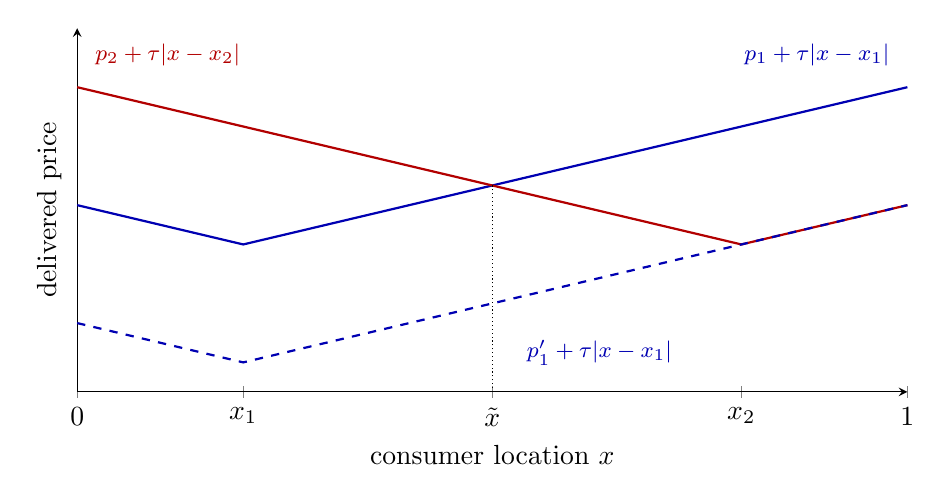
\begin{tikzpicture}
\begin{axis}[
  width=\linewidth, height=6.2cm,
  xmin=0, xmax=1, ymin=0.25, ymax=2.1,
  axis lines=left,
  xtick={0,0.2,0.5,0.8,1},
  xticklabels={$0$,$x_1$,$\tilde x$,$x_2$,$1$},
  ytick=\empty,
  xlabel={consumer location $x$},
  ylabel={delivered price},
  samples=201, domain=0:1,
  clip=false]
\addplot[thick, blue!70!black] {1 + abs(x - 0.2)};
\addplot[thick, red!70!black] {1 + abs(x - 0.8)};
\addplot[thick, dashed, blue!70!black] {0.4 + abs(x - 0.2)};
\draw[densely dotted] (axis cs:0.5,0.25) -- (axis cs:0.5,1.3);
\node[anchor=south west, font=\footnotesize, red!70!black] at (axis cs:0.01,1.86) {$p_2 + \tau|x - x_2|$};
\node[anchor=south east, font=\footnotesize, blue!70!black] at (axis cs:0.99,1.86) {$p_1 + \tau|x - x_1|$};
\node[anchor=north west, font=\footnotesize, blue!70!black] at (axis cs:0.53,0.56) {$p_1' + \tau|x - x_1|$};
\end{axis}
\end{tikzpicture}
\caption{Linear transport costs}
\end{subfigure}
\hfill
\begin{subfigure}[b]{0.48\textwidth}
\centering
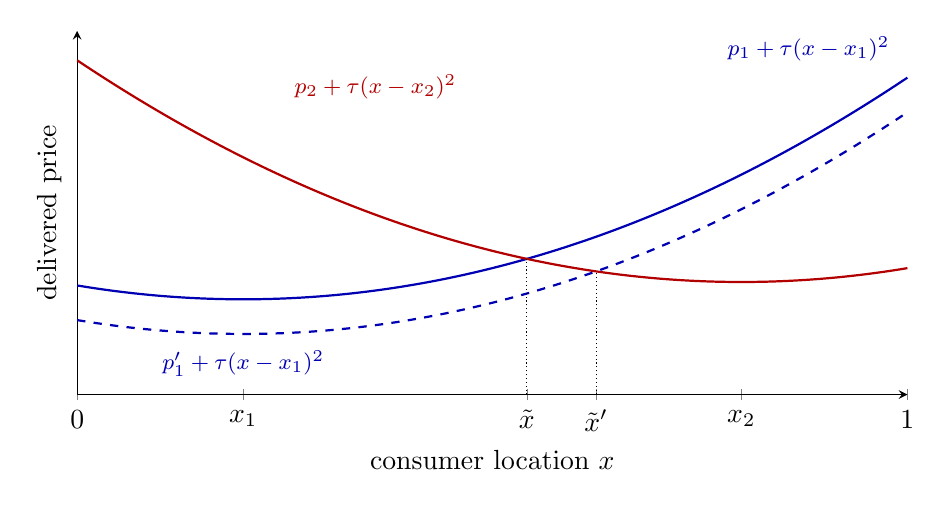
\begin{tikzpicture}
\begin{axis}[
  width=\linewidth, height=6.2cm,
  xmin=0, xmax=1, ymin=0.45, ymax=2.55,
  axis lines=left,
  xtick={0,0.2,0.5417,0.625,0.8,1},
  xticklabels={$0$,$x_1$,$\tilde x$,$\tilde x'$,$x_2$,$1$},
  ytick=\empty,
  xlabel={consumer location $x$},
  ylabel={delivered price},
  samples=201, domain=0:1,
  clip=false]
\addplot[thick, blue!70!black] {1 + 2*(x - 0.2)^2};
\addplot[thick, red!70!black] {1.1 + 2*(x - 0.8)^2};
\addplot[thick, dashed, blue!70!black] {0.8 + 2*(x - 0.2)^2};
\draw[densely dotted] (axis cs:0.5417,0.45) -- (axis cs:0.5417,1.234);
\draw[densely dotted] (axis cs:0.625,0.45) -- (axis cs:0.625,1.161);
\node[anchor=south west, font=\footnotesize, red!70!black] at (axis cs:0.25,2.1) {$p_2 + \tau(x - x_2)^2$};
\node[anchor=south east, font=\footnotesize, blue!70!black] at (axis cs:0.99,2.32) {$p_1 + \tau(x - x_1)^2$};
\node[anchor=north, font=\footnotesize, blue!70!black] at (axis cs:0.2,0.76) {$p_1' + \tau(x - x_1)^2$};
\end{axis}
\end{tikzpicture}
\caption{Quadratic transport costs}
\end{subfigure}
\caption{Delivered prices on Hotelling's line. Solid curves show each firm's price plus transport cost at the
initial prices, and the indifferent consumer $\tilde x$ is where they cross. In panel (a), with linear costs, firm 1
cuts its price to $p_1' = p_2 - \tau(x_2 - x_1)$ (dashed). Its schedule then coincides with firm 2's beyond $x_2$,
so firm 2's whole hinterland switches at once and demand jumps. In panel (b), with quadratic costs, a price cut (dashed)
moves the indifferent consumer continuously from $\tilde x$ to $\tilde x'$. Both panels use $x_1 = 0.2$ and $x_2 = 0.8$.
Panel (a) uses $\tau = 1$, $p_1 = p_2 = 1$ and $p_1' = 0.4$, and panel (b) uses $\tau = 2$, $p_1 = 1$, $p_2 = 1.1$ and
$p_1' = 0.8$.}
\label{fig:04-hotelling}
\end{figure}

\casehead{Firms at the ends} With $a = b = 0$, the middle case of \eqref{eq:04-hotelling-linear-demand} holds whenever
$|p_1 - p_2| \le \tau$. Firm 1 maximizes $(p_1 - c)M[\frac{1}{2} + \frac{p_2 - p_1}{2\tau}]$, a concave quadratic. Its
first-order condition is $\frac{1}{2} + \frac{p_2 - 2p_1 + c}{2\tau} = 0$, so the best response is
$p_1 = \frac{c + \tau + p_2}{2}$. Symmetry gives $p_1 = p_2 = c + \tau$, with $\tilde x = \frac{1}{2}$ and profits
$\frac{\tau M}{2}$. Undercutting to take the whole market requires $p_1 \le p_2 - \tau = c$, which earns nothing. The
markup equals the transport cost, so it vanishes as the products become perfect substitutes. This is the same
outcome as with quadratic costs at the ends (\cref{ex:06-hotelling}).

\casehead{Nonexistence when the firms are close} \Citet{Hotelling1929} argued that firms would cluster at the center
of the market, the \emph{principle of minimum differentiation}. \Citet{DAspremontGabszewiczThisse1979} showed that
the argument breaks down at the pricing stage. With linear costs, firms that are close have no pure-strategy price
equilibrium at all.

\begin{proposition}[Existence with linear transport costs]\label{prop:04-dgt}
Under \cref{ass:04-hotelling} with linear costs and $a, b \ge 0$, a pure-strategy price equilibrium exists if and only if
\begin{equation}\label{eq:04-dgt}
\Big(1 + \frac{a - b}{3}\Big)^2 \ge \frac{4}{3}(a + 2b)
\qquad\text{and}\qquad
\Big(1 + \frac{b - a}{3}\Big)^2 \ge \frac{4}{3}(b + 2a).
\end{equation}
When it exists, it is $p_1 = c + \tau(1 + \frac{a - b}{3})$ and $p_2 = c + \tau(1 + \frac{b - a}{3})$. With symmetric
locations, $a = b$, an equilibrium exists if and only if $a \le \frac{1}{4}$, and then $p_1 = p_2 = c + \tau$.
\end{proposition}

\begin{proof}
\emph{Step 1.} Any equilibrium lies in the middle region of \eqref{eq:04-hotelling-linear-demand}. Suppose firm 1
served the whole market, $p_1 < p_2 - \tau\Delta x$. Its profit is nonnegative only if $p_1 \ge c$. Firm 2 sells
nothing, yet it could charge any price in $(c, p_1 + \tau\Delta x)$, win some consumers and earn a positive profit.
That is a profitable deviation. The same argument rules out firm 2 serving everyone. At the boundary prices some
consumers are indifferent. Whichever way they break ties, one firm can gain by a small price change, so boundary
prices are not equilibria either.

\emph{Step 2.} In the middle region firm 1's profit is
$(p_1 - c)M[\frac{1 + a - b}{2} + \frac{p_2 - p_1}{2\tau}]$, a concave quadratic in $p_1$. Its first-order condition,
multiplied by $2\tau$, is $\tau(1 + a - b) + p_2 - 2p_1 + c = 0$. Firm 2's condition is symmetric:
\begin{equation*}
2p_1 - p_2 = c + \tau(1 + a - b), \qquad 2p_2 - p_1 = c + \tau(1 + b - a).
\end{equation*}
Adding twice the first equation to the second gives $3p_1 = 3c + \tau(3 + a - b)$, so
$p_1 = c + \tau(1 + \frac{a - b}{3})$, and by symmetry $p_2 = c + \tau(1 + \frac{b - a}{3})$. At these prices
$\tilde x = \frac{1 + a - b}{2} + \frac{b - a}{3} = \frac{3 + a - b}{6}$, and firm 1 earns
\begin{equation*}
\pi_1 = \tau\,\frac{3 + a - b}{3}\cdot M\,\frac{3 + a - b}{6} = \frac{M\tau}{2}\Big(1 + \frac{a - b}{3}\Big)^2 .
\end{equation*}
The candidate lies in the middle region if $|p_1 - p_2| = \frac{2\tau|a - b|}{3} < \tau\Delta x$. Take $a \ge b$. The
condition fails only if $5a + b \ge 3$, which with $b \le a$ requires $a \ge \frac{1}{2}$. Then the right side of
the second inequality in \eqref{eq:04-dgt} is at least $\frac{4}{3}$, while its left side is at most one. So
whenever \eqref{eq:04-dgt} holds, the candidate is interior.

\emph{Step 3.} Within the middle region the candidate is firm 1's best price. Prices that give firm 1 no
demand earn zero. The remaining deviation undercuts into the first region. There profit is $M(p_1 - c)$, which rises
with $p_1$, so the supremum is approached as $p_1$ rises to $p_2 - \tau\Delta x$. Its value is
\begin{equation*}
M\big(p_2 - \tau\Delta x - c\big) = M\tau\Big[1 + \frac{b - a}{3} - (1 - a - b)\Big] = \frac{2}{3}M\tau(a + 2b).
\end{equation*}
The candidate is a best response for firm 1 if and only if
$\frac{M\tau}{2}(1 + \frac{a - b}{3})^2 \ge \frac{2}{3}M\tau(a + 2b)$, which is the first inequality in
\eqref{eq:04-dgt}. The second inequality is the same condition for firm 2. By Steps 1 and 2 no other price pair
can be an equilibrium. With $a = b$ both inequalities read $1 \ge 4a$.
\end{proof}

The undercutting deviation drives the result. Holding firm 2's location fixed, firm 1's profit at the candidate
prices rises as firm 1 moves toward the center, with slope $\frac{M\tau}{3}(1 + \frac{a - b}{3})$. Its undercutting
payoff $\frac{2}{3}M\tau(a + 2b)$ rises faster, with slope $\frac{2}{3}M\tau$, and it also rises with $b$. When both
firms move inward together, $a = b$, the candidate profit stays at $\frac{M\tau}{2}$ while the undercutting payoff
$2M\tau a$ grows. When the firms are close, each prefers to undercut
the other and capture the whole line, and no pair of prices is stable. Mixed-strategy equilibria still exist, but
they are of little use for comparative statics (\cref{sec:04-existence-problem}). Hotelling's principle of minimum
differentiation therefore fails as a result about the location-price game. \Citet{CaplinNalebuff1991} make the same
point from the side of their existence theorem. Hotelling's distance utility is not linear in the consumer's
location, and the resulting discontinuity of demand is inconsistent with their assumptions (\cref{thm:04-cn-existence}).

\subsection{Quadratic transport costs and the location-price game}\label{sec:04-hotelling-quad}

\Citet{DAspremontGabszewiczThisse1979} restored existence by making transport costs quadratic. A consumer at $x$
then pays $p_j + \tau(x - x_j)^2$. The cost difference between the two firms is linear in $x$, so the
indifferent consumer moves continuously with prices, as panel (b) of \cref{fig:04-hotelling} shows. We now allow any
real $a$ and $b$ with $a + b < 1$, so that firms may also locate outside the line.

\begin{proposition}[Hotelling with quadratic costs]\label{prop:04-hotelling}
Let \cref{ass:04-hotelling} hold with quadratic costs and suppose that $|a - b| < 3$, so that the indifferent
consumer at the prices below lies strictly inside $[0,1]$.
\begin{enumerate}[label=(\roman*)]
\item The unique price equilibrium is
\begin{equation}\label{eq:04-hotelling-quad-prices}
p_1 = c + \tau(1 - a - b)\Big(1 + \frac{a - b}{3}\Big), \qquad p_2 = c + \tau(1 - a - b)\Big(1 + \frac{b - a}{3}\Big),
\end{equation}
with $q_1 = M\frac{3 + a - b}{6}$ and $\pi_1 = \frac{M\tau}{18}(1 - a - b)(3 + a - b)^2$.
\item In the first stage of a game in which firms choose locations and then prices,
\begin{equation}\label{eq:04-hotelling-location}
\frac{\dd\pi_1}{\dd a} = -\frac{M\tau}{18}(3 + a - b)(1 + 3a + b) < 0 \qquad\text{for all } a, b \ge 0 .
\end{equation}
If locations are restricted to $[0,1]$, the unique location equilibrium is $x_1 = 0$, $x_2 = 1$ (maximal
differentiation), with prices $c + \tau$.
\item If locations are unrestricted, the location equilibrium is $x_1 = -\frac{1}{4}$ and $x_2 = \frac{5}{4}$.
\end{enumerate}
\end{proposition}

\begin{proof}
(i) Let $\Delta x = 1 - a - b$. The indifferent consumer solves $p_1 + \tau(x - a)^2 = p_2 + \tau(x - 1 + b)^2$. The
quadratic terms $\tau x^2$ cancel, leaving
\begin{equation*}
2\tau x\,(1 - b - a) = p_2 - p_1 + \tau\big[(1 - b)^2 - a^2\big] = p_2 - p_1 + \tau(1 - a - b)(1 - b + a),
\end{equation*}
so that
\begin{equation*}
\tilde x = \frac{1 + a - b}{2} + \frac{p_2 - p_1}{2\tau\Delta x} = a + \frac{\Delta x}{2} + \frac{p_2 - p_1}{2\tau\Delta x}.
\end{equation*}
Consumers to the left of $\tilde x$ buy from firm 1, so $q_1 = M\tilde x$ when $\tilde x \in [0,1]$. Firm 1 maximizes
$(p_1 - c)M\tilde x$. Its first-order condition, multiplied by $\frac{2\tau\Delta x}{M}$, is
$\tau\Delta x(1 + a - b) + p_2 - 2p_1 + c = 0$. Firm 2 sells $M(1 - \tilde x)$ and has the symmetric condition.
The system is
\begin{equation*}
2p_1 - p_2 = c + \tau\Delta x(1 + a - b), \qquad 2p_2 - p_1 = c + \tau\Delta x(1 + b - a).
\end{equation*}
Adding twice the first to the second gives $3p_1 = 3c + \tau\Delta x(3 + a - b)$, which is
\eqref{eq:04-hotelling-quad-prices}. Then $p_2 - p_1 = \frac{2}{3}\tau\Delta x(b - a)$, so
$\tilde x = \frac{1 + a - b}{2} + \frac{b - a}{3} = \frac{3 + a - b}{6}$. Profit is
$(p_1 - c)M\tilde x = \tau\Delta x\frac{3 + a - b}{3}\cdot M\frac{3 + a - b}{6}$. Demand is continuous, and where
positive it is the minimum of $M$ and a linear function, hence log-concave. By \cref{lem:04-logconcave} profit is
quasi-concave in own price, so the first-order conditions give best responses, and the prices
\eqref{eq:04-hotelling-quad-prices} are an equilibrium.

The best-response map is not a contraction on all prices. When $p_2$ is high, firm 1's best response takes the
whole market, $\tilde x = 1$, and then rises one for one with $p_2$. We therefore prove uniqueness directly. In an
equilibrium with $0 < \tilde x < 1$, profits are differentiable in own prices, so both first-order conditions hold.
The linear system above then has the single solution \eqref{eq:04-hotelling-quad-prices}. Suppose instead that an
equilibrium had $\tilde x \geq 1$, so that firm 2 sells nothing. If $\tilde x > 1$, firm 1 could raise its price
slightly and still serve everyone, so $\tilde x = 1$. If $p_2 > c$, firm 2 could cut its price slightly and earn a
positive profit, so $p_2 \leq c$. With $\tilde x = 1$, firm 1's price is
$p_1 = p_2 - \tau\Delta x(1 - a + b) \leq c - \tau\Delta x(1 - a + b)$. A small rise in $p_1$ changes firm 1's
profit at the rate $M\big[1 - \frac{p_1 - c}{2\tau\Delta x}\big]$, so firm 1 gains from it unless
$p_1 - c \geq 2\tau\Delta x$. Both bounds on $p_1 - c$ hold only if $a - b \geq 3$, which the assumption rules out.
The case $\tilde x \leq 0$ is symmetric and requires $b - a \geq 3$. The equilibrium is therefore unique.

(ii) By the envelope theorem, the effect of $a$ on $\pi_1$ at the equilibrium of (i) has two parts. The direct
effect holds both prices fixed: $(p_1 - c)M\frac{\partial\tilde x}{\partial a}$. The strategic effect works through
the rival's price: $(p_1 - c)M\frac{\partial\tilde x}{\partial p_2}\frac{\dd p_2}{\dd a}$. Firm 1's own price response
has no first-order effect. At the equilibrium, with $\frac{p_2 - p_1}{2\tau\Delta x^2} = \frac{b - a}{3\Delta x}$,
\begin{equation*}
\frac{\partial\tilde x}{\partial a} = \frac{1}{2} + \frac{p_2 - p_1}{2\tau\Delta x^2} = \frac{3 - 5a - b}{6\Delta x},
\qquad
\frac{\partial\tilde x}{\partial p_2} = \frac{1}{2\tau\Delta x},
\qquad
\frac{\dd p_2}{\dd a} = -\frac{\tau(4 - 2a)}{3}.
\end{equation*}
The last derivative follows from differentiating $p_2 = c + \frac{\tau}{3}(1 - a - b)(3 + b - a)$, which gives
$\frac{\tau}{3}[-(3 + b - a) - (1 - a - b)] = -\frac{\tau}{3}(4 - 2a)$. Adding the two effects,
\begin{equation*}
\frac{\dd\pi_1}{\dd a} = (p_1 - c)M\Big[\frac{3 - 5a - b}{6\Delta x} - \frac{4 - 2a}{6\Delta x}\Big]
= -(p_1 - c)M\frac{1 + 3a + b}{6\Delta x}.
\end{equation*}
Substituting $p_1 - c = \frac{\tau\Delta x(3 + a - b)}{3}$ gives \eqref{eq:04-hotelling-location}, which is negative
for $a, b \ge 0$. Each firm therefore wants to move away from the center for any location of its rival. On $[0,1]$
the unique equilibrium is $a = b = 0$, and (i) gives prices $c + \tau$.

(iii) Without restrictions, the location first-order conditions are $1 + 3a + b = 0$ for firm 1 and
$1 + 3b + a = 0$ for firm 2. Their solution is $a = b = -\frac{1}{4}$, so $x_1 = -\frac{1}{4}$ and
$x_2 = 1 + \frac{1}{4} = \frac{5}{4}$. Given $b = -\frac{1}{4}$, the derivative \eqref{eq:04-hotelling-location} is
positive for $a < -\frac{1}{4}$ and negative above, so $a = -\frac{1}{4}$ is firm 1's best location.
\end{proof}

The two effects in the proof have a clear meaning. The direct effect is positive as long as $5a + b < 3$. Moving
toward the center at given prices takes consumers from the rival. The strategic effect is negative, because moving
closer makes the products better substitutes and lowers the rival's price. The strategic effect always wins.
\Citet{ShakedSutton1982} call this \emph{relaxing price competition through product differentiation}. Firms give up
market share at given prices to soften the price war that would follow. The result is
\emph{maximal differentiation}, the opposite of Hotelling's conjecture.

Equilibrium differentiation is excessive from the social point of view. With a covered market and inelastic unit
demand, prices are transfers, and welfare depends only on transport costs. A planner who places two products to
minimize average transport cost chooses $\frac{1}{4}$ and $\frac{3}{4}$, with average cost
$2\int_0^{\frac{1}{2}}\tau(x - \frac{1}{4})^2\dd x = \frac{\tau}{48}$. Firms at the ends impose
$2\int_0^{\frac{1}{2}}\tau x^2\dd x = \frac{\tau}{12}$, four times as much. When firms may locate outside the line, they move
even farther apart, to $-\frac{1}{4}$ and $\frac{5}{4}$. \Citet[Section 7.1.1]{Tirole1988} gives a textbook treatment.

\casehead{Minimal differentiation with fixed prices} Hotelling's principle does hold when prices cannot compete.
\Citet[Section 7.1.3]{Tirole1988} shows this with Hotelling's own location game at an exogenous price.

\begin{proposition}[Location choice at a fixed price]\label{prop:04-hotelling-fixed}
Let consumers be uniform on $[0,1]$ with mass $M$ and buy one unit each from the nearest firm. Two firms sell at a
common exogenous price $p > c$ and choose locations $x_1 = a$ and $x_2 = 1 - b$, splitting demand equally if they
locate at the same point. The unique equilibrium places both firms at $\frac{1}{2}$.
\end{proposition}

\begin{proof}
Prices and margins are fixed, so each firm maximizes its demand. Suppose first that $a < 1 - b$. Firm 1 serves its
hinterland and half of the consumers between the firms, so its demand is
\begin{equation*}
q_1 = M\Big[a + \frac{1 - b - a}{2}\Big] = M\,\frac{1 + a - b}{2} .
\end{equation*}
It rises with $a$, so firm 1 gains by moving toward its rival, and the same holds for firm 2. Any equilibrium therefore
has $a = 1 - b$. Suppose the common location is $x < \frac{1}{2}$. Each firm sells $\frac{M}{2}$. If firm 2 moves to
$x + e$ with small $e > 0$, it serves every consumer to the right of $x + \frac{e}{2}$, which gives
$M(1 - x - \frac{e}{2}) > \frac{M}{2}$. So $x < \frac{1}{2}$ is not an equilibrium, and the same argument rules out
$x > \frac{1}{2}$. At $x = \frac{1}{2}$, a firm that moves to any $x' \neq \frac{1}{2}$ serves only the consumers on
its side of the midpoint between $x'$ and $\frac{1}{2}$. That is less than half of the market, so neither firm
deviates.
\end{proof}

The products are socially too close. With linear costs, the average distance is $\frac{1}{4}$ when both firms sit
at the center and $\frac{1}{8}$ at the efficient locations $\frac{1}{4}$ and $\frac{3}{4}$. The contrast with
\cref{prop:04-hotelling} isolates the role of prices. Firms differentiate to soften price competition, and without
price competition they have no reason to. \citet[Section 7.1.3]{Tirole1988} groups the forces that work against
maximal differentiation into three categories. The first is the location of demand. Firms want to be where consumers
are, and when demand is concentrated around a few poles they cluster there. Tirole's examples are ice cream parlors
and bookstores near universities. The second is positive externalities among firms. On the cost side these include
shared installations and sources of raw materials. On the demand side, consumer search draws stores together, as
with the furniture stores of a single Paris street. The third is the absence of price competition, as in the game
above. Airline fares in the United States before deregulation and the prices of gasoline and books in France were
once set outside the market. Resale price maintenance has the same effect. Tirole adds that fixed-price location
models may explain why political platforms cluster at the center.

Two connections close this subsection. First, quadratic costs satisfy the linearity assumption of
\cref{thm:04-cn-existence}. Expanding the square gives $-\tau(x - x_j)^2 = -\tau x^2 + 2\tau x\,x_j - \tau x_j^2$. The
first term is common to all products and drops out, and the second is linear in the consumer's type $x$. With
uniform types, which have a log-concave density, an equilibrium exists for any locations
\citep{CaplinNalebuff1991}. Second, heterogeneity in tastes can bring minimum differentiation back.
\Citet{DePalmaEtAl1985} add a logit taste shock to Hotelling's linear transport costs. Demand becomes smooth, and with
enough taste heterogeneity relative to $\tau$, both firms locate at the center of the market. Their title states the
result: the principle of minimum differentiation holds under sufficient heterogeneity.

\subsection{Salop's circle, free entry and excess variety}\label{sec:04-salop}

\Citet{Salop1979} removed the ends of the line by placing consumers on a circle. Without ends there are no
hinterlands, and symmetric configurations with any number of firms are natural. This makes the circle the standard
model of entry with differentiated products.

\begin{proposition}[Salop's circle]\label{prop:04-salop}
Let a mass $M$ of consumers be uniform on a circle of circumference one, buy one unit each, and have a high enough
reservation value that the market is covered. $N$ firms are equally spaced, with marginal cost $c$, fixed cost
$\phi$ and linear transport cost $\tau$.
\begin{enumerate}[label=(\roman*)]
\item There is a symmetric price equilibrium with $p = c + \frac{\tau}{N}$, in which each firm earns
$\frac{\tau M}{N^2} - \phi$.
\item Treating $N$ as continuous, free entry yields $N^* = \sqrt{\frac{\tau M}{\phi}}$ firms.
\item The number of firms that minimizes fixed plus transport costs is $N^o = \frac{1}{2}\sqrt{\frac{\tau M}{\phi}}$.
Hence $N^* = 2N^o$.
\end{enumerate}
\end{proposition}

\begin{proof}
(i) Take a firm that charges $p$ while its two neighbors, each at distance $\frac{1}{N}$, charge $\bar p$. A consumer
at distance $d$ from the firm, on the arc toward a neighbor, is indifferent when
$p + \tau d = \bar p + \tau(\frac{1}{N} - d)$, that is, at $d = \frac{1}{2N} + \frac{\bar p - p}{2\tau}$. The firm serves
the arcs on both sides, so its demand is
\begin{equation*}
q = 2Md = M\Big[\frac{1}{N} + \frac{\bar p - p}{\tau}\Big] \qquad\text{for } |\bar p - p| \le \frac{\tau}{N}.
\end{equation*}
In this range profit $(p - c)q - \phi$ is a concave quadratic. Its first-order condition is
$\frac{1}{N} + \frac{\bar p - p}{\tau} - \frac{p - c}{\tau} = 0$. At a symmetric point $p = \bar p$, it gives
$p = c + \frac{\tau}{N}$. Each firm sells $\frac{M}{N}$ and earns $\frac{\tau}{N}\cdot\frac{M}{N} - \phi$. To take its
neighbor's whole market, a firm would have to price at $\bar p - \frac{\tau}{N} = c$, which earns no variable profit.
A price above $\bar p + \frac{\tau}{N}$ sells nothing. So no deviation outside the range is profitable.

(ii) Free entry drives profit to zero: $\frac{\tau M}{N^2} = \phi$, so $N^* = \sqrt{\frac{\tau M}{\phi}}$.

(iii) With $N$ equally spaced firms, each consumer travels to the nearest firm. Distances are uniform on
$[0, \frac{1}{2N}]$, so the average distance is $\frac{1}{4N}$ and total transport cost is $\frac{\tau M}{4N}$.
Prices are transfers because the market is covered. The planner minimizes $N\phi + \frac{\tau M}{4N}$. The
first-order condition $\phi - \frac{\tau M}{4N^2} = 0$ gives $N^o = \frac{1}{2}\sqrt{\frac{\tau M}{\phi}}$.
\end{proof}

\begin{figure}[htbp]
\centering
\begin{tikzpicture}
\def\R{2.3}
\draw[thick] (0,0) circle (\R);
\draw[line width=6pt, blue!25] (60:\R) arc (60:120:\R);
\foreach \a in {90,30,150,210,270,330} {\fill (\a:\R) circle (2.6pt);}
\foreach \a in {60,120} {\draw[thick] (\a:\R-0.18) -- (\a:\R+0.18);}
\node[anchor=south] at (90:\R+0.2) {firm $j$, price $p$};
\node[anchor=south west] at (30:\R+0.12) {firm $j+1$, price $\bar p$};
\node[anchor=south east] at (150:\R+0.12) {firm $j-1$, price $\bar p$};
\draw[<->, >=Stealth] (90:\R-0.55) arc (90:30:\R-0.55);
\node at (58:\R-1.05) {$\frac{1}{N}$};
\draw[<->, >=Stealth] (90:\R-1.0) arc (90:120:\R-1.0);
\node at (106:\R-1.45) {$\frac{1}{2N}$};
\node[align=center, font=\small] at (0,-0.45) {consumers uniform\\on the circle};
\end{tikzpicture}
\caption{Salop's circle with $N = 6$ equally spaced firms. Firm $j$ serves the shaded arc between the two
indifferent consumers (tick marks). At symmetric prices each indifferent consumer is at distance
$d = \frac{1}{2N}$ from firm $j$, so the firm's market has length $\frac{1}{N}$. A price cut by firm $j$ moves
both tick marks outward and takes customers from its two neighbors only.}
\label{fig:04-salop}
\end{figure}

\Cref{fig:04-salop} shows the structure. Each firm competes only with its two neighbors, and its markup
$\frac{\tau}{N}$ falls as the circle fills up. The market provides twice the efficient number of products. The reason
is the balance of two externalities \citep{Spence1976,DixitStiglitz1977,MankiwWhinston1986}. An entrant creates
variety: consumers near its location travel less. It does not capture this whole benefit in its profit, which pushes
toward too little entry. An entrant also steals business from incumbents, which pushes toward too much entry. On the
circle the market is covered, so every unit the entrant sells is taken from a rival. At $N^*$ the entrant's private
gain, its variable profit $\frac{\tau M}{N^2} = \phi$, is four times the social gain $\frac{\tau M}{4N^2} = \frac{\phi}{4}$
in saved transport costs. Business stealing dominates. \Cref{prop:02-mw-excess} gives the corresponding result for
homogeneous goods.

\begin{remark}[Coverage and touching markets]\label{rem:04-salop-coverage}
\Cref{prop:04-salop} assumes that every consumer buys. Let $\bar u$ be the reservation value. The consumer farthest
from a firm is at distance $\frac{1}{2N}$ and pays $c + \frac{\tau}{N} + \frac{\tau}{2N} = c + \frac{3\tau}{2N}$, so the
equilibrium requires $\bar u \ge c + \frac{3\tau}{2N}$. At free entry $\frac{\tau}{N^*} = \sqrt{\frac{\tau\phi}{M}}$, and
the condition becomes
\begin{equation*}
\frac{3}{2}\sqrt{\frac{\tau\phi}{M}} \le \bar u - c
\quad\Longleftrightarrow\quad
\phi \le \bar\phi = \frac{4M(\bar u - c)^2}{9\tau}
\end{equation*}
\citep[Section 7.1.2]{Tirole1988}. With larger fixed costs fewer firms enter, and the consumer halfway between two
firms would not buy at the price of the proposition. \Citet{Salop1979} studies this case. Suppose the neighbors charge
$\bar p = \bar u - \frac{\tau}{2N}$, so that the consumer halfway between two firms is just willing to buy. A firm that
raises its price loses customers to the outside good. Its demand is then $\frac{2M(\bar u - p)}{\tau}$, with slope
$-\frac{2M}{\tau}$. A firm that cuts its price takes customers from its neighbors, with the demand of the proof and
slope $-\frac{M}{\tau}$. Demand therefore has a kink at $\bar p$. At sales of $\frac{M}{N}$, a price rise does not pay if
$\frac{M}{N} \le \frac{2M}{\tau}(\bar p - c)$, and a price cut does not pay if $\frac{M}{N} \ge \frac{M}{\tau}(\bar p - c)$.
So $\bar p$ is an equilibrium price whenever
\begin{equation*}
\frac{\tau}{N} \le \bar u - c \le \frac{3\tau}{2N} .
\end{equation*}
Free entry requires $G(N) \equiv (\bar u - c - \frac{\tau}{2N})\frac{M}{N} = \phi$. In this regime
$G'(N) = \frac{M}{N^2}\big[\frac{\tau}{N} - (\bar u - c)\big] \le 0$, and $G$ also falls with $\tau$. A higher fixed cost
or a higher transport cost therefore lowers the number of firms, and the price $\bar u - \frac{\tau}{2N}$ falls with it.
In the competitive regime of the proposition both changes raise the price. \Citet[Section 7.1.2,
Exercise 7.4]{Tirole1988} calls such results a priori counterintuitive. The explanation is that the price is pinned
by the reservation value of the consumer halfway between two firms. When firms are farther apart, that consumer
travels farther and can pay less.
\end{remark}

The factor of two depends on linear costs. With quadratic costs $\tau d^2$ on the circle, the same steps give the
markup $\frac{\tau}{N^2}$ and free-entry number $N^* = (\frac{\tau M}{\phi})^{\frac{1}{3}}$. Average transport cost is
$\frac{\tau}{12N^2}$, so the optimum is $N^o = (\frac{\tau M}{6\phi})^{\frac{1}{3}}$ and $\frac{N^*}{N^o} = 6^{\frac{1}{3}} \approx 1.82$.
Entry is still excessive. The dimension of the space matters more. \Citet{CaplinNalebuff1991} discuss
\citet{Stiglitz1986}, who places firms on a grid in $L$ dimensions with quadratic transport costs, so each firm has
$2L$ neighbors. Demand becomes more elastic as $L$ grows, profits fall, and fewer firms can cover the entry cost.
Yet consumers have farther to travel in higher dimensions, so the efficient number of firms per unit area rises.
Stiglitz concludes that low-dimensional markets have excess diversity and high-dimensional markets too little
\citep[Section 8.3 and n.~21]{CaplinNalebuff1991}. Caplin and Nalebuff show that, with quadratic costs, the
symmetric solution of the first-order conditions in his model is indeed an equilibrium. \Cref{fig:04-voronoi}
shows the two-dimensional analogue of the circle's market areas.

The circle fixes locations by assumption. \Citet[Section 7.1.2]{Tirole1988} discusses three extensions. First, equal
spacing is a natural guess given maximal differentiation on the line. \Citet{Economides1989} justifies it with
quadratic costs in a game where firms choose entry, then locations, then prices, and a symmetric free-entry
equilibrium exists. Tirole cites the 1984 working-paper version. Second, firms may enter in sequence, and then an
early entrant's location shapes later choices. \Citet{PrescottVisscher1977} studied sequential location on the line.
Third, one firm may sell several brands and crowd the product space so that no entrant fits, especially when it can
preempt. \Citet[p.~1283, n.~4]{AndersonDePalmaNesterov1995} add that the known results for the circle all suggest
substantial overentry at every level of fixed costs.

The welfare comparison has been taken to data. \Citet{BerryWaldfogel1999} estimate how listening and advertising
revenue vary with the number of radio stations in 135 US metropolitan markets and recover fixed costs from a
free-entry condition. In the 1996 working-paper version on which we rely, the welfare loss from free entry relative
to the social optimum is 40 percent of industry revenue. This calculation leaves out the value of programming to
listeners. Advertisers pay 4.5 cents per hour for a marginal listener. The authors compute that free entry would be
optimal if programming were worth more than three times that amount to the marginal listener.

\subsection{Symmetric logit oligopoly and entry*}\label{sec:04-logit-entry}

The symmetric logit gives a useful contrast with the circle. Every product competes with every other, and each new
product brings a new taste shock and hence new variety.

\begin{proposition}[Symmetric logit oligopoly and entry]\label{prop:04-logit-entry}
Let $N \ge 2$ single-product firms sell products with common quality $\tilde\delta$ and marginal cost $c$ to a mass
$M$ of consumers with logit demand and no outside good. Each firm pays a fixed cost $\phi$.
\begin{enumerate}[label=(\roman*)]
\item The symmetric price equilibrium has markup $p - c = \frac{N}{\alpha(N - 1)}$, and each firm earns
$\frac{M}{\alpha(N - 1)} - \phi$. With an outside good, the markup is $\frac{1}{\alpha(1 - s)}$, with $s$ each
firm's share.
\item Treating $N$ as continuous, free entry yields $N^* = 1 + \frac{M}{\alpha\phi}$.
\item Total surplus is $TS(N) = \frac{M}{\alpha}\ln N + M\big(\frac{\tilde\delta}{\alpha} - c\big) - N\phi$, up to a
constant. It is maximized at $N^o = \frac{M}{\alpha\phi}$, so $N^* = N^o + 1$.
\end{enumerate}
\end{proposition}

\begin{proof}
(i) With no outside good, the shares are $\frac{e^{\delta_j}}{\sum_ke^{\delta_k}}$, and at symmetric prices $s = \frac{1}{N}$.
The first-order condition of a single-product firm, $\alpha(p - c)(1 - s) = 1$, is derived as in
\cref{prop:04-logit-markup}, which does not use the outside good. With $s = \frac{1}{N}$ it gives
$p - c = \frac{1}{\alpha(1 - \frac{1}{N})} = \frac{N}{\alpha(N - 1)}$. Each firm sells $\frac{M}{N}$ and earns
$\frac{N}{\alpha(N-1)}\cdot\frac{M}{N} - \phi$. With an outside good, \cref{prop:04-logit-markup} applies directly.
(ii) Setting profit to zero gives $\alpha(N - 1)\phi = M$.
(iii) By \cref{prop:04-logit-entropy}, consumer surplus is $\frac{M}{\alpha}\ln\sum_{k=1}^Ne^{\tilde\delta - \alpha p}$ up
to a constant. At symmetric prices this equals $\frac{M}{\alpha}\ln N + \frac{M\tilde\delta}{\alpha} - Mp$. Total
profit is $M(p - c) - N\phi$. In the sum the price cancels, because every consumer buys and payments are
transfers. The derivative $TS'(N) = \frac{M}{\alpha N} - \phi$ vanishes at $N^o = \frac{M}{\alpha\phi}$, and $TS$ is
concave. Comparing with (ii) gives $N^* = N^o + 1$.
\end{proof}

The logit market also has too many products, but only one too many. The relative excess
$\frac{N^* - N^o}{N^o} = \frac{\alpha\phi}{M}$ vanishes as the market grows, whereas on the circle it is always
100 percent. The reason lies in the social value of the marginal product. In the logit it is $\frac{M}{\alpha N}$,
which falls slowly with $N$, because each product brings its own taste shock. On the circle it is
$\frac{\tau M}{4N^2}$, which falls fast, because a new product only shortens the trips of nearby consumers. The
entrant's private gain, $\frac{M}{\alpha(N - 1)}$, exceeds the social gain by only
$\frac{M}{\alpha N(N - 1)}$. Business stealing is weak because the logit treats variety itself as valuable.
\Citet[p.~49]{MankiwWhinston1986} isolate the two forces at work. Business stealing pushes toward excessive entry,
as in homogeneous-good markets. Product diversity pushes the other way, because the entrant creates surplus through
variety that it does not capture as profit. With the CES form and equilibrium notion of \citet{Spence1976}, the
diversity effect always dominates and entry is insufficient. They also give examples in which business stealing
always dominates. The symmetric logit of \cref{prop:04-logit-entry} is another such case, with an excess of one firm.
For the CES, \citet{DixitStiglitz1977} show that the market can provide too few or too many products, depending on
preferences (\cref{sec:04-repcons-monocomp}).

\casehead{General i.i.d.\ tastes} \Citet{AndersonDePalmaNesterov1995} ask how far the logit's verdict extends. They
keep the symmetric discrete choice structure, with the demand side of \citet{PerloffSalop1985}, but let the taste
shocks have any log-concave density. The following proposition collects the pieces we need, in our notation.

\begin{proposition}[Symmetric oligopoly with i.i.d.\ tastes]\label{prop:04-adn}
A mass $M$ of consumers each buy one unit of the product that maximizes $u_{ij} = y - p_j + \epsilon_{ij}$. The shocks
$\epsilon_{ij}$ are i.i.d.\ across consumers and products, with density $f_\epsilon$ and distribution function $F_\epsilon$
on $(\underline e, \bar e)$ and a finite mean. There are $N \ge 2$ single-product firms with marginal cost $c$ and
fixed cost $\phi$.
\begin{enumerate}[label=(\roman*)]
\item Demand for product $i$ is
\begin{equation}\label{eq:04-adn-demand}
q_i = M\int f_\epsilon(x)\prod_{j \ne i}F_\epsilon(p_j - p_i + x)\,\dd x .
\end{equation}
\item The unique candidate for a symmetric equilibrium has the markup
\begin{equation}\label{eq:04-adn-markup}
p - c = \frac{1}{\Theta(N)}, \qquad \Theta(N) = N(N - 1)\int f_\epsilon(x)^2F_\epsilon(x)^{N-2}\,\dd x .
\end{equation}
\item At equal prices, an $(N+1)$th product raises total surplus by $M\int F_\epsilon(x)^N[1 - F_\epsilon(x)]\,\dd x - \phi$.
Its profit in the symmetric equilibrium with $N + 1$ firms is $\frac{M}{(N + 1)\Theta(N + 1)} - \phi$.
\item If $\epsilon_{ij}$ is type-I extreme value with scale $\frac{1}{\alpha}$, then $\Theta(N) = \frac{\alpha(N - 1)}{N}$,
the markup is $\frac{N}{\alpha(N - 1)}$, and the surplus gain in (iii) is $\frac{M}{\alpha}\ln\frac{N + 1}{N} - \phi$.
\item If $F_\epsilon(x) = 1 - e^{-\lambda_\epsilon(x - \underline e)}$ on $[\underline e, \infty)$ with $\lambda_\epsilon > 0$,
then $\Theta(N) = \lambda_\epsilon$ for every $N$. The surplus gain and the profit in (iii) are both
$\frac{M}{\lambda_\epsilon(N + 1)} - \phi$.
\end{enumerate}
\end{proposition}

\begin{proof}
(i) Fix a consumer and write $\epsilon_k$ for her shock on product $k$. She buys $i$ when
$y - p_i + \epsilon_i > y - p_j + \epsilon_j$ for every $j \ne i$. Given $\epsilon_i = x$, this requires
$\epsilon_j < p_j - p_i + x$ for every $j \ne i$. By independence the conditional probability is
$\prod_{j \ne i}F_\epsilon(p_j - p_i + x)$. Integrating over the density of $x$ gives \eqref{eq:04-adn-demand}. Ties
have probability zero.

(ii) Differentiate \eqref{eq:04-adn-demand} with respect to $p_i$ and set all prices equal. Each of the $N - 1$ factors
contributes $-f_\epsilon(x)F_\epsilon(x)^{N-2}$, so
\begin{equation*}
\frac{\partial q_i}{\partial p_i} = -M(N - 1)\int f_\epsilon(x)^2F_\epsilon(x)^{N-2}\,\dd x = -\frac{M\,\Theta(N)}{N} .
\end{equation*}
At equal prices $q_i = \frac{M}{N}$. The first-order condition $q_i + (p_i - c)\frac{\partial q_i}{\partial p_i} = 0$
becomes $\frac{M}{N} = (p - c)\frac{M\,\Theta(N)}{N}$, which has the single solution \eqref{eq:04-adn-markup}.

(iii) Every consumer buys and prices are transfers, so at equal prices total surplus is $M(y - c)$ plus
$M\E[\max_j\epsilon_{ij}]$ minus total fixed costs. The maximum of $N$ shocks has distribution function $F_\epsilon^N$.
Integrating by parts, with boundary terms that vanish because the mean is finite,
\begin{equation*}
\E\big[\max_{j \le N + 1}\epsilon_{ij}\big] - \E\big[\max_{j \le N}\epsilon_{ij}\big]
= \int x\,\dd\big(F_\epsilon^{N+1} - F_\epsilon^N\big)(x) = \int F_\epsilon(x)^N\big[1 - F_\epsilon(x)\big]\,\dd x .
\end{equation*}
With $N + 1$ firms, each sells $\frac{M}{N + 1}$ at the markup $\frac{1}{\Theta(N + 1)}$, which gives the profit.

(iv) Here $F_\epsilon(x) = \exp(-e^{-\alpha x})$ and $f_\epsilon(x) = \alpha e^{-\alpha x}F_\epsilon(x)$, so
$f_\epsilon^2F_\epsilon^{N-2} = \alpha^2e^{-2\alpha x}\exp(-Ne^{-\alpha x})$. Substitute $u = e^{-\alpha x}$, with
$\dd x = -\frac{\dd u}{\alpha u}$:
\begin{equation*}
\int f_\epsilon(x)^2F_\epsilon(x)^{N-2}\,\dd x = \alpha\int_0^\infty ue^{-Nu}\,\dd u = \frac{\alpha}{N^2},
\qquad\text{so}\qquad
\Theta(N) = \frac{\alpha(N - 1)}{N} .
\end{equation*}
For the surplus, $F_\epsilon(x)^N = \exp\big(-e^{-\alpha(x - \frac{\ln N}{\alpha})}\big)$. The maximum of $N$ shocks is
therefore extreme value with location $\frac{\ln N}{\alpha}$, and its mean rises by $\frac{1}{\alpha}\ln\frac{N + 1}{N}$
when $N$ rises by one.

(v) Let $v = F_\epsilon(x)$, so that $f_\epsilon(x) = \lambda_\epsilon(1 - v)$ and $\dd v = \lambda_\epsilon(1 - v)\,\dd x$. Then
\begin{equation*}
\int f_\epsilon^2F_\epsilon^{N-2}\,\dd x = \lambda_\epsilon\int_0^1(1 - v)v^{N-2}\,\dd v
= \lambda_\epsilon\Big[\frac{1}{N - 1} - \frac{1}{N}\Big] = \frac{\lambda_\epsilon}{N(N - 1)},
\end{equation*}
so $\Theta(N) = \lambda_\epsilon$. Likewise $\int F_\epsilon^N(1 - F_\epsilon)\,\dd x = \frac{1}{\lambda_\epsilon}\int_0^1v^N\,\dd v =
\frac{1}{\lambda_\epsilon(N + 1)}$, and the profit is $\frac{M}{(N + 1)\lambda_\epsilon} - \phi$.
\end{proof}

Part (iv) is the integer version of \cref{prop:04-logit-entry}. The $(N+1)$th product adds
$\frac{M}{\alpha}\ln(1 + \frac{1}{N})$ to surplus and earns $\frac{M}{\alpha N}$, and $\ln(1 + \frac{1}{N}) < \frac{1}{N}$.
The general results of \citet{AndersonDePalmaNesterov1995} rest on log-concavity. Utility is linear in the vector of
shocks, whose joint density $\prod_jf_\epsilon(\epsilon_{ij})$ is log-concave when $f_\epsilon$ is. The theorem of
\citet{CaplinNalebuff1991} then makes profit quasi-concave, so the candidate in (ii) is an equilibrium (p.~1285,
\cref{thm:04-cn-existence}). Their Proposition 1 (p.~1285) shows that log-concavity also makes $\Theta(N)$
nondecreasing, so markups do not rise with entry. Revenue per firm then falls with $N$, and the free-entry number of
firms is unique. Their Theorem 1 (p.~1287) is the main result. With log-concave tastes and unit demands, the profit of
an extra firm is never below its social value, so the market never provides too little variety. Corollary 1
(p.~1289) shows that equilibrium and optimum coincide for every fixed cost only for the exponential-tail
distributions of part (v) and their mirror images. For the densities of their example held fixed, the equilibrium
number of firms is about the optimum plus one as fixed costs vanish (p.~1290), as in the logit. For a general fixed
density only the ratio of the two numbers tends to one, a result \citet[p.~1283]{AndersonDePalmaNesterov1995}
credit to \citet{DeneckereRothschild1992}. Overentry can still be large. For
each optimal number of firms they choose a log-concave density, and as fixed costs vanish the ratio of the
equilibrium to the optimal number tends to $r^* > 1.097$ (p.~1290). That is almost 10 percent excess entry even with
very many firms. When individual demand responds to price, entry can fall short of the optimum subject to zero
profits, but by at most one firm (their Theorem 2, p.~1294).

The logit's verdict depends on taking the taste shocks literally. If they are a statistical device, the term
$\frac{M}{\alpha}\ln N$ overstates the value of variety, and the true optimum may be far below $N^o$. This is the
``too many characteristics'' problem of \cref{sec:04-spaces-drawbacks} in its welfare form. It is also why models of
entry and variety that use logit demand need care before their welfare conclusions are trusted.

\subsection{Vertical differentiation and quality choice}\label{sec:04-vertical-quality}

In the models so far consumers disagree about which product is best at equal prices. In a \emph{vertical} model
they agree: at equal prices every consumer ranks products the same way. Consumers differ only in how much they value
quality relative to money. Consumer $i$ has utility $v_ix_j - p_j$ from product $j$ with quality $x_j$. The taste for
quality $v_i$ is uniform on $[\underline v, \bar v]$ with mass $M$. Dividing utility by $v_i$ gives
$x_j - \frac{1}{v_i}p_j$, the vertical model $u_{ij} = \delta_j - \nu_ip_j$ of \cref{ch:discrete} with
$\delta_j = x_j$ and price sensitivity $\nu_i = \frac{1}{v_i}$.

\begin{proposition}[Price and quality competition with vertical differentiation]\label{prop:04-vertical}
Two firms with a common marginal cost $c \ge 0$ sell qualities $x_1 < x_2$. Assume $\bar v > 2\underline v$ and the
coverage condition $c + \frac{1}{3}(\bar v - 2\underline v)(\bar x - \underline x) \le \underline v\,\underline x$, where
qualities lie in $[\underline x, \bar x]$.
\begin{enumerate}[label=(\roman*)]
\item The price equilibrium is
\begin{equation}\label{eq:04-vertical-prices}
p_1 = c + \frac{(\bar v - 2\underline v)(x_2 - x_1)}{3}, \qquad p_2 = c + \frac{(2\bar v - \underline v)(x_2 - x_1)}{3},
\end{equation}
with cutoff type $\hat v = \frac{\bar v + \underline v}{3}$ and profits
$\pi_1 = \frac{M(\bar v - 2\underline v)^2(x_2 - x_1)}{9(\bar v - \underline v)}$ and
$\pi_2 = \frac{M(2\bar v - \underline v)^2(x_2 - x_1)}{9(\bar v - \underline v)}$.
\item If firms first choose qualities in $[\underline x, \bar x]$ at no cost and then set prices, the equilibrium
qualities are $\underline x$ and $\bar x$.
\end{enumerate}
\end{proposition}

\begin{proof}
(i) Let $\Delta x = x_2 - x_1$. Type $v$ prefers quality 2 when $vx_2 - p_2 > vx_1 - p_1$, that is, when
$v > \hat v = \frac{p_2 - p_1}{\Delta x}$. Under coverage every type buys, so with density $\frac{M}{\bar v - \underline v}$,
\begin{equation*}
q_1 = M\frac{\hat v - \underline v}{\bar v - \underline v}, \qquad q_2 = M\frac{\bar v - \hat v}{\bar v - \underline v}.
\end{equation*}
Firm 1 maximizes $(p_1 - c)q_1$. Since $\frac{\partial\hat v}{\partial p_1} = -\frac{1}{\Delta x}$, its first-order
condition is $\hat v - \underline v - \frac{p_1 - c}{\Delta x} = 0$, or $p_2 - 2p_1 = \underline v\Delta x - c$. Firm 2's
condition is $\bar v - \hat v - \frac{p_2 - c}{\Delta x} = 0$, or $2p_2 - p_1 = \bar v\Delta x + c$. The first gives
$p_2 = 2p_1 + \underline v\Delta x - c$. Substituting into the second gives $3p_1 = 3c + (\bar v - 2\underline v)\Delta x$,
and then $p_2 = c + \frac{(2\bar v - \underline v)\Delta x}{3}$. The cutoff is
$\hat v = \frac{p_2 - p_1}{\Delta x} = \frac{\bar v + \underline v}{3}$, which lies strictly inside $(\underline v, \bar v)$
because $\bar v > 2\underline v$. Profits follow from the margins $p_j - c$ and from
$\hat v - \underline v = \frac{\bar v - 2\underline v}{3}$ and $\bar v - \hat v = \frac{2\bar v - \underline v}{3}$. Coverage
requires that the lowest type buy, $\underline vx_1 \ge p_1$. The left side is smallest and the right side largest at
$x_1 = \underline x$ and $x_2 = \bar x$, where the assumed condition makes it hold. A firm that raised its price
enough to lose low types would face demand no larger than the covered formula, so the candidate remains optimal.

(ii) Both profits are proportional to $\Delta x$. Given $x_2 = \bar x$, the low-quality firm's profit
$\propto \bar x - x_1$ is largest at $x_1 = \underline x$. Choosing $x_1 = \bar x$ would make the products identical and
drive both prices to marginal cost, and leapfrogging is impossible. Given $x_1 = \underline x$, the high-quality firm's
profit $\propto x_2 - \underline x$ is largest at $\bar x$. So $(\underline x, \bar x)$ is an equilibrium. In any
configuration with $\underline x < x_1$ or $x_2 < \bar x$, one firm can raise $\Delta x$ and its profit, and equal
qualities yield zero profits. So the only equilibria assign $\underline x$ to one firm and $\bar x$ to the other.
\end{proof}

\begin{figure}[htbp]
\centering
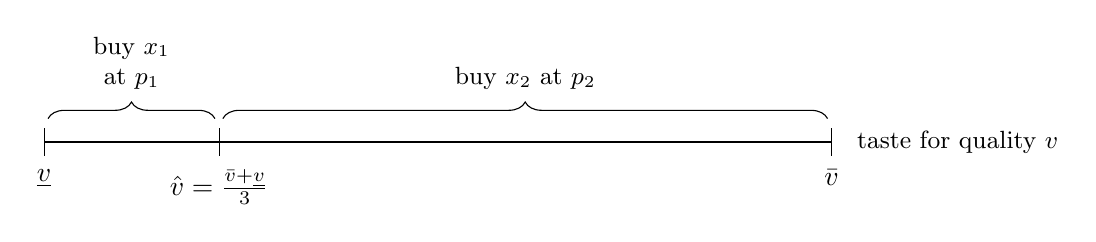
\begin{tikzpicture}[x=1cm,y=1cm]
\draw[thick] (0,0) -- (10,0);
\draw (0,0.18) -- (0,-0.18);
\draw (10,0.18) -- (10,-0.18);
\draw (2.222,0.18) -- (2.222,-0.18);
\node[below] at (0,-0.22) {$\underline v$};
\node[below] at (10,-0.22) {$\bar v$};
\node[below] at (2.222,-0.22) {$\hat v = \frac{\bar v + \underline v}{3}$};
\draw[decorate, decoration={brace, amplitude=6pt}] (0.05,0.3) -- (2.17,0.3)
  node[midway, above=7pt, align=center, font=\small] {buy $x_1$\\at $p_1$};
\draw[decorate, decoration={brace, amplitude=6pt}] (2.27,0.3) -- (9.95,0.3)
  node[midway, above=7pt, align=center, font=\small] {buy $x_2$ at $p_2$};
\node[anchor=west, font=\small] at (10.2,0) {taste for quality $v$};
\end{tikzpicture}
\caption{Market segments in the vertical duopoly of \cref{prop:04-vertical}, drawn for $\underline v = 1$ and
$\bar v = 4$. Consumers with a high taste for quality buy the high-quality product. The cutoff
$\hat v = \frac{\bar v + \underline v}{3}$ does not depend on the two qualities.}
\label{fig:04-vertical}
\end{figure}

\Cref{fig:04-vertical} shows the segments. The force behind part (ii) is the one we saw on Hotelling's line. Closer
qualities mean fiercer price competition, so firms differentiate as much as they can
\citep{GabszewiczThisse1979,ShakedSutton1982}. The high-quality firm charges more, sells more and earns more. Both
markups and profits scale with the quality gap $x_2 - x_1$, and they vanish when the products are identical.

\Citet[Section 7.5.1]{Tirole1988} draws out two further points. First, part (ii) has two equilibria, which differ
only in which firm takes the top quality. If one firm chooses its quality first, it takes $\bar x$ and leaves
$\underline x$ to its rival, so the equilibrium is unique. Since $\pi_2 > \pi_1$, each firm would like to move first.
With a cost of introducing a quality and growing demand, this becomes a preemption race, in which firms trade the
gain from leadership against the cost of entering too early. Second, maximal differentiation is not robust. If the
lowest feasible quality is so low that the coverage condition fails, the low-quality firm loses the bottom of the
market and no longer wants the lowest quality. The effect is stronger when marginal costs differ across qualities,
which already softens price competition. The principle of differentiation itself survives.

\begin{remark}[Natural oligopoly]\label{rem:04-natural-oligopoly}
The condition $\bar v > 2\underline v$ requires enough dispersion in tastes. If $\bar v \le 2\underline v$, formula
\eqref{eq:04-vertical-prices} would give $p_1 \le c$. The equilibrium then has $p_1 = c$ and the high-quality firm
serving every consumer at the limit price $p_2 = c + \underline v(x_2 - x_1)$, the highest price at which the lowest
type still prefers quality 2. To see this, write $m_2 = p_2 - c$. At $p_1 = c$, firm 2's profit for
$m_2 > \underline v\Delta x$ is $m_2M\frac{\bar v\Delta x - m_2}{(\bar v - \underline v)\Delta x}$. Its slope at
$m_2 = \underline v\Delta x$ is $M\frac{\bar v - 2\underline v}{\bar v - \underline v} \le 0$, and it is concave, so firm 2
does not raise its price further. With any positive fixed cost, only one firm enters, however large $M$ is. This is
the simplest instance of the finiteness property of \citet{ShakedSutton1983}, which \citet[Section 7.5.1]{Tirole1988}
states as follows. Let quality $x$ cost $c(x)$ per unit. Suppose that, if every quality were sold at its unit cost,
all consumers would buy the highest quality. Then at most a finite number of firms can have positive market shares,
whatever the relative sizes of demand and entry costs. Price competition among the high-quality firms leaves no room
for low qualities. The condition requires unit cost to rise slowly with quality. Shaked and Sutton therefore expect
finiteness when the burden of quality improvement falls mainly on research and development or other fixed costs,
rather than on labor and materials. On the circle, by contrast, the number of firms grows without bound as fixed
costs vanish. \Cref{ch:discrete} estimates the vertical demand model, and \citet{Bresnahan1987} applies it to the 1955
automobile price war.
\end{remark}

\subsection{From address models to discrete choice}\label{sec:04-location-bridge}

Location models are characteristics-space models with one or two characteristics and no idiosyncratic taste
shock. Substitution is local. On the line and the circle a product competes only with its neighbors, and in the
vertical model only with the products just above and below it in quality. Adding a product close to an existing one
adds little value, since the gain on the circle is the saved transport cost of nearby consumers. Logit-type models
sit at the opposite extreme. Every product competes with every other, IIA holds, and each new product adds value
through its own taste shock (\cref{sec:04-spaces-drawbacks}). The two classes share a formal structure.
Expanding the square in a quadratic ideal-point model turns it into a random coefficients model, as shown in
\cref{prop:06-idealpoint}. The pure characteristics model of \citet{BerryPakes2007} keeps the local substitution of
address models while allowing many characteristics and estimation from market data (\cref{ch:discrete}). Random
coefficient logit models (\cref{ch:blp}) sit between the extremes. They generate local substitution through
correlated tastes while keeping the logit shock.

Location models also frame empirical work on product choice. In the location and quality games above, firms choose
positions in anticipation of price competition. Mergers change these incentives. \Citet{Sweeting2010} studies how
radio stations reposition their formats after mergers (\cref{ch:mergers}). The estimation of such product choice
models builds on the equilibrium theory of this section.
